%-----------------------------------------------------------------------------%
\chapter{\babTiga}
\label{bab:3}
%-----------------------------------------------------------------------------%
Bab ini memaparkan metode penelitian yang digunakan untuk mengembangkan sistem deteksi kecurangan akademik berbasis kecerdasan buatan pada platform Moodle. Metodologi penelitian dirancang melalui pendekatan sistematis yang dimulai dari pemahaman masalah, perancangan solusi, hingga implementasi dan evaluasi. Pembahasan mencakup enam fase utama: (1) analisis kebutuhan dan studi literatur, (2) akuisisi dan persiapan data, (3) perancangan data artifisial dengan \textit{ground truth} terkontrol, (4) pengembangan \textit{pipeline preprocessing} dan ekstraksi fitur, (5) pelatihan model \textit{ensemble machine learning}, dan (6) evaluasi komprehensif pada data riil dan artifisial.

\begin{figure}[htbp]
    \centering
    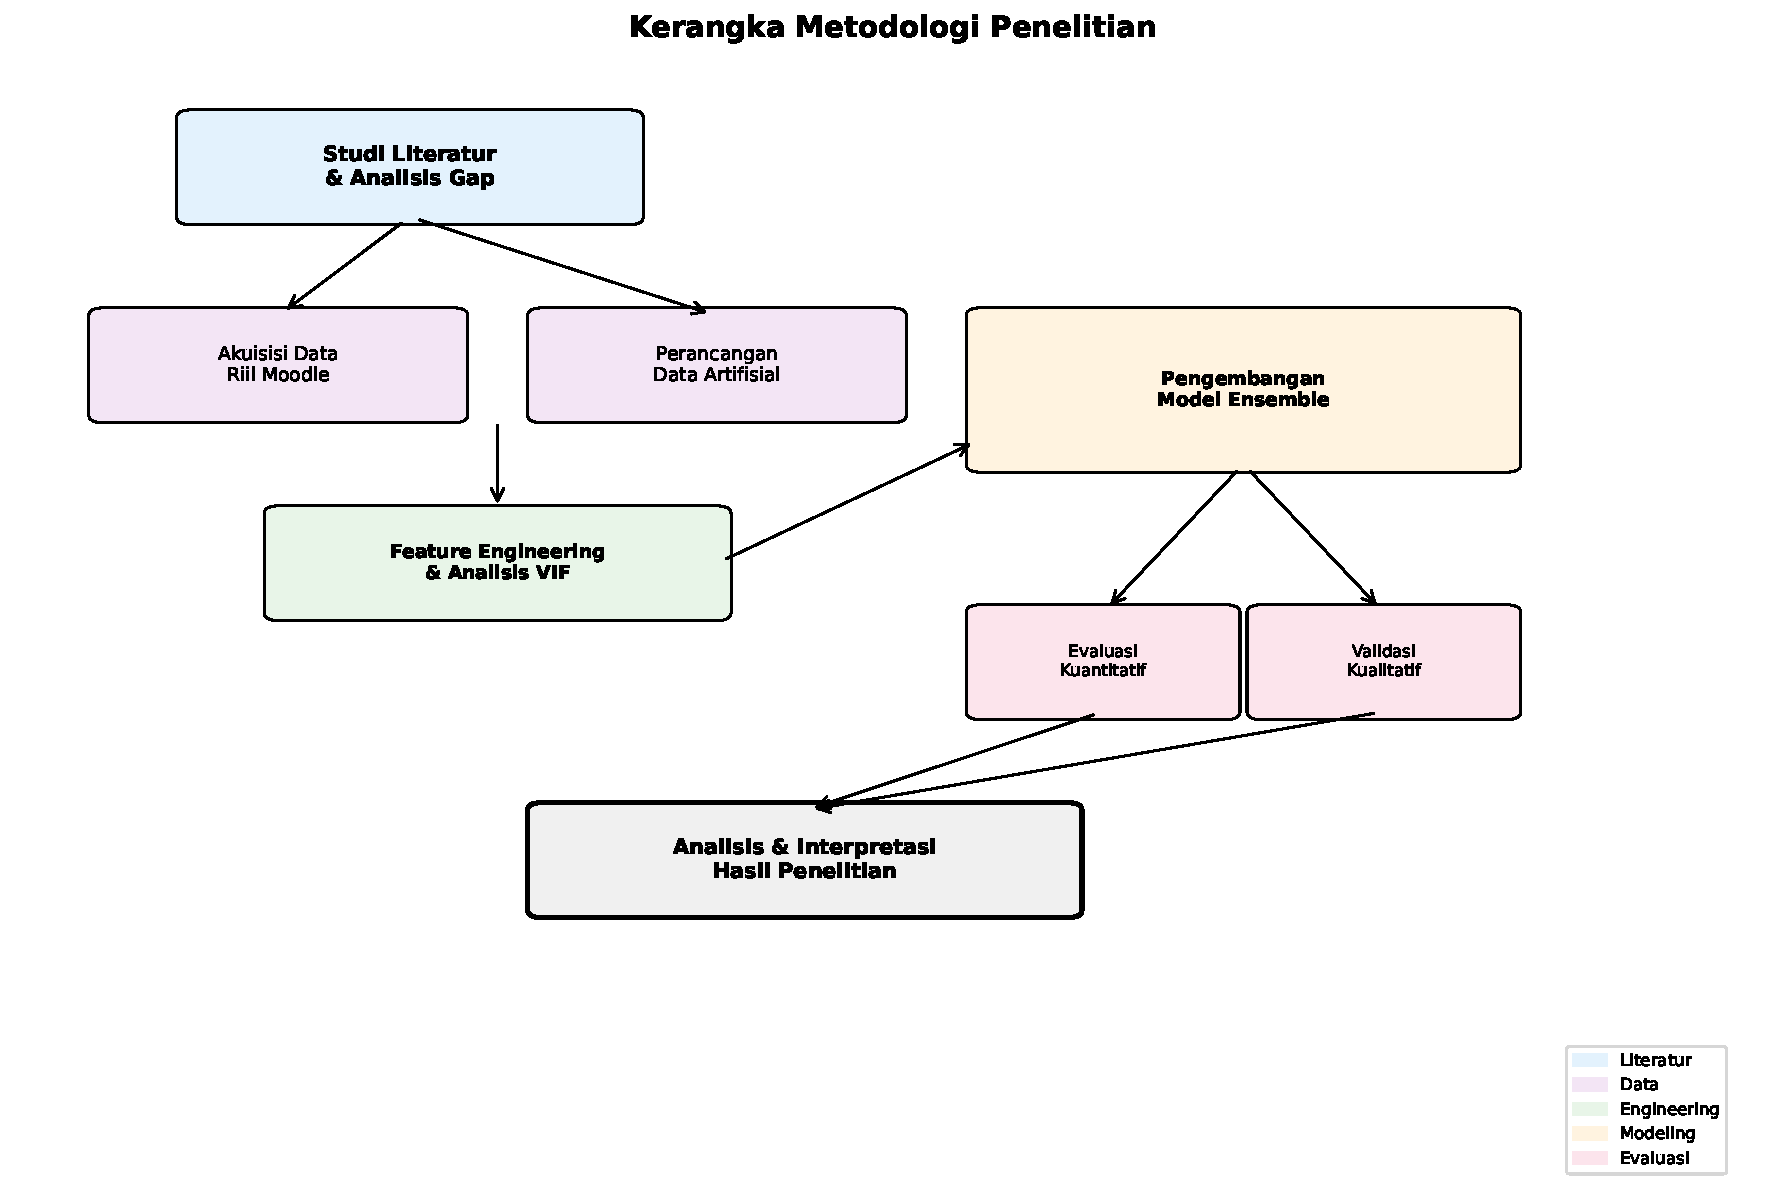
\includegraphics[width=0.95\textwidth]{newfigures/research_methodology_stages.pdf}
    \caption{Kerangka Metodologi Penelitian Deteksi Kecurangan}
    \label{fig:research_stages}
\end{figure}

Gambar \ref{fig:research_stages} menunjukkan kerangka metodologi penelitian yang terdiri dari enam fase utama yang saling berkaitan. Setiap fase dirancang secara spesifik untuk menjawab pertanyaan penelitian yang telah dirumuskan pada Bab 1. Fase 1 mengidentifikasi pola-pola kecurangan akademik melalui studi literatur. Fase 2 dan 3 mempersiapkan data pelatihan dengan \textit{ground truth} yang terkontrol. Fase 4 mentransformasi data mentah menjadi fitur-fitur bermakna. Fase 5 mengembangkan model deteksi menggunakan pendekatan \textit{ensemble}. Fase 6 mengevaluasi efektivitas model pada skala operasional.

\begin{figure}[htbp]
    \centering
    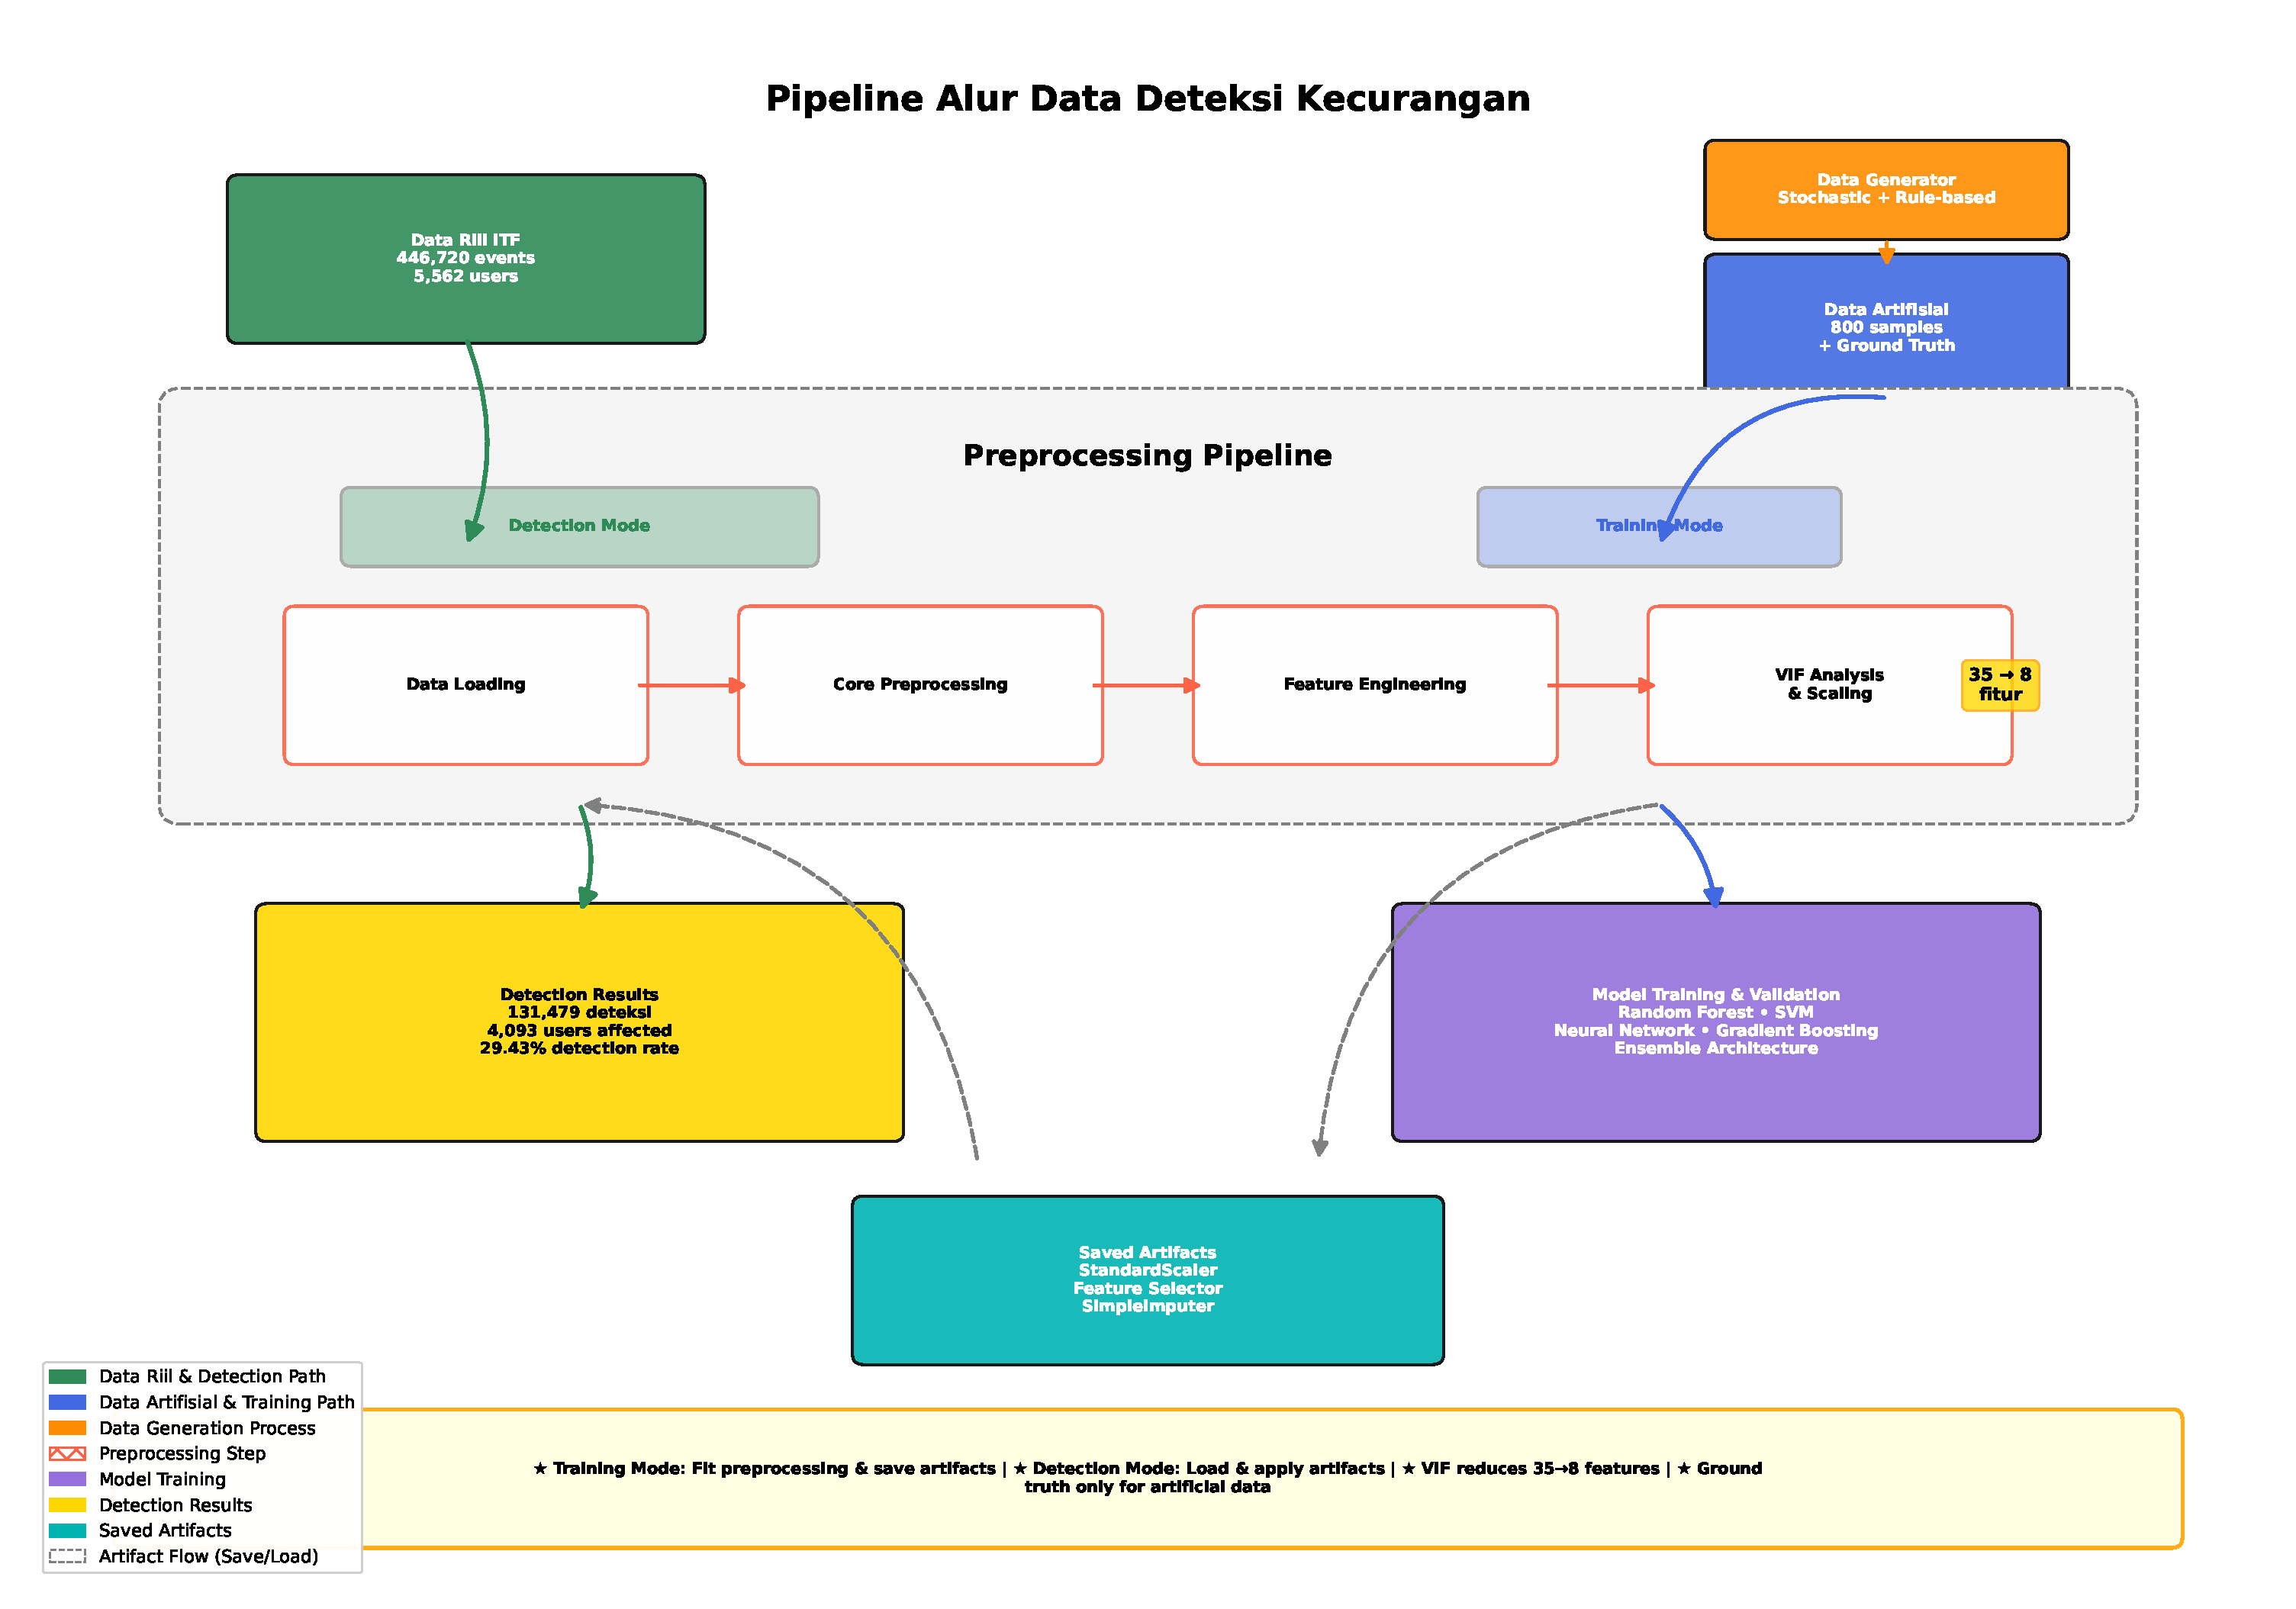
\includegraphics[width=0.98\textwidth]{newfigures/technical_pipeline_flow_final.pdf}
    \caption{Arsitektur Pipeline Teknis: Alur Pemrosesan Data dari Log Mentah hingga Deteksi Kecurangan dengan Dual-Mode Processing}
    \label{fig:technical_pipeline}
\end{figure}

Gambar \ref{fig:technical_pipeline} menerjemahkan kerangka metodologi konseptual menjadi implementasi teknis yang detail. \textit{Pipeline} dimulai dari dua sumber data yang berbeda karakteristiknya: \textbf{Data Riil ITF} yang berisi 446.720 \textit{events} dari aktivitas nyata mahasiswa Fasilkom UI, dan \textbf{Data Artifisial} dengan 800 sampel terkontrol yang dilengkapi \textit{ground truth} untuk pelatihan model. 

Perbedaan krusial terletak pada strategi pemrosesan: data artifisial diproses dalam \textit{Training Mode} untuk membangun dan menyimpan \textit{artifacts} pembelajaran (\textit{scaler}, \textit{feature selector}, \textit{imputer}), sementara data riil menggunakan \textit{Detection Mode} yang memanfaatkan \textit{artifacts} tersebut untuk konsistensi transformasi. \textit{Pipeline} berhasil mereduksi kompleksitas dari 35 fitur awal menjadi 8 fitur stabil melalui analisis \textit{Variance Inflation Factor} (VIF), menghasilkan model \textit{ensemble} yang mendeteksi 131.479 percobaan ujian mencurigakan (29,43\% dari total).

Kombinasi kedua diagram memberikan pemahaman menyeluruh: Gambar \ref{fig:research_stages} menyediakan peta konseptual untuk memandu pembaca melalui logika penelitian, sedangkan Gambar \ref{fig:technical_pipeline} memberikan \textit{blueprint} teknis untuk reproduksi penelitian. Integrasi pendekatan \textit{top-down} (konseptual) dan \textit{bottom-up} (teknis) ini memastikan transparansi metodologi yang dapat dipertanggungjawabkan secara ilmiah.

%-----------------------------------------------------------------------------%
%-----------------------------------------------------------------------------%
\section{Desain Penelitian dan Hipotesis}
\label{sec:desainPenelitian}
%-----------------------------------------------------------------------------%
Penelitian ini mengadopsi pendekatan eksperimental dengan kombinasi data artifisial dan riil untuk mengembangkan sistem deteksi kecurangan yang \textit{robust} (kokoh) dan dapat diimplementasikan dalam skala institusional. Desain penelitian dirancang secara sistematis untuk menjawab pertanyaan penelitian utama: bagaimana mengembangkan sistem deteksi kecurangan otomatis yang akurat untuk platform Moodle menggunakan pendekatan \textit{machine learning}?

\subsection{Alur Tahapan Penelitian}
\label{subsec:alurTahapanPenelitian}
Penelitian dilakukan melalui enam tahapan sistematis yang saling terkait:

\begin{enumerate}
    \item \textbf{Fase 1 - Analisis Kebutuhan dan Studi Literatur:} Mengidentifikasi pola-pola kecurangan akademik dalam pembelajaran daring melalui \textit{review} sistematis literatur. Fase ini menghasilkan pemahaman mendalam tentang karakteristik perilaku curang dan metode deteksi yang telah ada.
    
    \item \textbf{Fase 2 - Akuisisi Data Log Moodle:} Mengumpulkan data log aktivitas dari platform Moodle Fasilkom UI dengan total 446.720 \textit{events}. Data melalui proses anonimisasi untuk menjaga privasi pengguna.
    
    \item \textbf{Fase 3 - Perancangan Data Artifisial:} Mengembangkan generator data artifisial yang mensimulasikan 800 skenario ujian dengan parameter kecurangan terkontrol. Setiap skenario dilengkapi \textit{ground truth} untuk validasi model.
    
    \item \textbf{Fase 4 - Pengembangan \textit{Pipeline Preprocessing}:} Mengimplementasikan sistem ekstraksi dan transformasi fitur yang menghasilkan 35 fitur awal, kemudian direduksi menjadi 8 fitur stabil melalui analisis VIF.
    
    \item \textbf{Fase 5 - Pelatihan Model \textit{Ensemble}:} Melatih kombinasi algoritma \textit{Random Forest}, SVM, \textit{Neural Network}, dan \textit{Gradient Boosting} dengan optimasi \textit{hyperparameter} sistematis.
    
    \item \textbf{Fase 6 - Evaluasi Multi-Aspek:} Menguji model pada data artifisial (evaluasi kuantitatif) dan mengaplikasikan pada data riil (evaluasi kualitatif) untuk memvalidasi efektivitas deteksi.
\end{enumerate}

Setiap fase dirancang dengan \textit{output} yang jelas dan terukur, memungkinkan evaluasi progres penelitian secara objektif. Pendekatan iteratif diterapkan di mana hasil evaluasi dapat memicu perbaikan pada fase-fase sebelumnya.

\subsection{Hipotesis Penelitian}
\label{subsec:hipotesisPenelitian}
Berdasarkan studi literatur dan analisis awal, penelitian ini menguji empat hipotesis utama:

\textbf{H1: Deteksi Pola Kolaborasi}\\
Kolaborasi kecurangan akan menghasilkan pola similaritas yang dapat dideteksi dalam tiga dimensi: navigasi (urutan pengerjaan soal), \textit{timing} (pola waktu), dan jawaban (kesamaan respons). Hipotesis ini memprediksi tingkat akurasi deteksi $>90\%$ untuk kasus dengan koordinasi tinggi.

\textbf{H2: Superioritas Model Gabungan}\\
Model \textit{ensemble} (model gabungan) yang mengintegrasikan beberapa algoritma akan memberikan performa superior (peningkatan \textit{F1-score} minimal 5\%) dibandingkan model tunggal dalam mendeteksi berbagai strategi kecurangan yang heterogen.

\textbf{H3: \textit{Threshold} Ukuran Dataset}\\
Dataset dengan minimal 500-1000 sampel diperlukan untuk mencapai performa deteksi yang optimal (akurasi $>95\%$). Peningkatan ukuran dataset akan menghasilkan peningkatan performa yang signifikan hingga mencapai titik saturasi.

\textbf{H4: Generalisasi Model}\\
Model yang dilatih pada data artifisial dengan parameter terkontrol dapat menggeneralisasi dengan baik pada data riil skala besar, dengan tingkat deteksi yang konsisten dengan prevalensi kecurangan dalam literatur (20-40\%).

Keempat hipotesis ini akan diuji secara empiris melalui eksperimen yang dirancang dalam metodologi penelitian, dengan hasil pengujian disajikan pada Bab 4.

%-----------------------------------------------------------------------------%
%-----------------------------------------------------------------------------%
\section{Strategi Akuisisi dan Persiapan Data}
\label{sec:strategiAkuisisiData}
%-----------------------------------------------------------------------------%
Penelitian ini mengimplementasikan strategi \textit{dual-data} yang menggabungkan kekuatan data riil (validitas eksternal) dan data artifisial (kontrol internal) untuk mengoptimalkan pengembangan model deteksi kecurangan. Strategi ini memungkinkan pelatihan model dengan \textit{ground truth} yang terkontrol sambil mempertahankan kemampuan generalisasi pada kondisi operasional nyata.

%-----------------------------------------------------------------------------%
\section{Arsitektur Pipeline Preprocessing: Dari Log Mentah ke Fitur Terstruktur}
\label{sec:pipelinePreprocessing}
%-----------------------------------------------------------------------------%
\textit{Pipeline preprocessing} data merupakan komponen krusial yang mentransformasi log mentah Moodle menjadi representasi fitur yang siap untuk \textit{machine learning}. Sesuai dengan Fase 4 pada Gambar \ref{fig:research_stages}, \textit{pipeline} ini memproses kedua jenis data (riil dan artifisial) melalui empat modul terintegrasi dengan strategi \textit{dual-mode} yang memastikan konsistensi transformasi.

\subsection{Komponen dan Alur Kerja Pipeline}
\label{sec:komponenPipeline}

\textit{Pipeline preprocessing} dirancang dengan arsitektur modular yang terdiri dari empat komponen utama:

\textbf{Modul I - \textit{Data Loading} dan Validasi:} \\
Modul pertama bertanggung jawab memuat data dari berbagai tabel Moodle dengan validasi komprehensif. Tabel-tabel utama yang diproses meliputi mdl\_quiz\_attempts (percobaan ujian), mdl\_question\_attempt\_steps (langkah pengerjaan), dan mdl\_question\_attempt\_step\_data (detail jawaban). Validasi mencakup pemeriksaan tipe data, konsistensi referensial antar tabel, dan penanganan nilai yang hilang atau \textit{corrupt}. \textit{Output} modul ini adalah dataset terintegrasi yang siap untuk \textit{preprocessing} lanjutan.

\textbf{Modul II - \textit{Core Preprocessing} dan Normalisasi:} \\
Modul kedua melakukan pembersihan dan normalisasi fundamental. Proses utama meliputi: (1) unifikasi \textit{timestamp} ke format POSIX untuk konsistensi temporal, (2) penggabungan tabel-tabel terkait melalui \textit{foreign key} untuk membentuk \textit{event log} komprehensif, (3) \textit{filtering} data berdasarkan kriteria penelitian seperti status \textit{quiz completion}, dan (4) penghapusan duplikasi dan anomali data. Modul ini menghasilkan \textit{clean dataset} dengan struktur yang konsisten.

\textbf{Modul III - \textit{Feature Engineering} Multi-Dimensi:} \\
Modul ketiga mengekstraksi fitur-fitur \textit{behavioral} dari \textit{event log} yang telah dibersihkan. Ekstraksi fitur dilakukan dalam empat kategori:
\begin{itemize}
    \item \textbf{\textit{Intra-Attempt Features}:} Mengukur karakteristik dalam satu percobaan ujian seperti \textit{total duration}, \textit{number of actions}, dan \textit{step duration statistics}
    \item \textbf{\textit{Sequential Features}:} Menangkap pola urutan seperti \textit{navigation patterns}, \textit{revisit counts}, \textit{linearity measures}, dan entropi navigasi
    \item \textbf{\textit{Similarity Features}:} Menghitung kemiripan antar pengguna menggunakan \textit{Levenshtein distance} untuk navigasi dan korelasi statistik untuk \textit{timing patterns}
    \item \textbf{\textit{Comparative Features}:} Menormalkan perilaku individual terhadap populasi menggunakan transformasi \textit{z-score}
\end{itemize}

\textbf{Modul IV - \textit{Feature Selection} dan \textit{Optimization}:} \\
Modul terakhir melakukan optimasi fitur melalui beberapa tahap:
\begin{itemize}
    \item \textbf{\textit{Missing Value Imputation}:} Menggunakan \textit{SimpleImputer} dengan strategi \textit{mean} untuk fitur numerik
    \item \textbf{\textit{Multicollinearity Analysis}:} Menghitung \textit{Variance Inflation Factor} (VIF) dan mengeliminasi fitur dengan VIF $>10$
    \item \textbf{\textit{Variance Filtering}:} Menghilangkan fitur dengan \textit{variance} $<0,01$ yang tidak informatif
    \item \textbf{\textit{Standardization}:} Menerapkan \textit{StandardScaler} untuk normalisasi distribusi fitur
\end{itemize}

\subsection{Strategi \textit{Dual-Mode Processing}}
\label{sec:dualModeStrategy}

Inovasi kunci dalam \textit{pipeline} adalah implementasi \textit{dual-mode processing} yang membedakan pemrosesan data \textit{training} dan \textit{detection}:

\textbf{\textit{Training Mode} untuk Data Artifisial:} \\
Dalam \textit{mode training}, \textit{pipeline} melakukan \textit{fitting} terhadap data artifisial dan menyimpan semua \textit{transformation artifacts} ke direktori preprocessing/\textit{artifacts}/. \textit{Artifacts} yang disimpan meliputi: (1) \textit{fitted imputer} untuk menangani \textit{missing value}, (2) \textit{fitted scaler} dengan parameter \textit{mean} dan \textit{standard deviation}, (3) \textit{feature selector} dengan daftar fitur terpilih, dan (4) \textit{metadata} transformasi untuk \textit{reproducibility}. Mode ini memungkinkan eksplorasi parameter \textit{preprocessing} optimal melalui eksperimen terkontrol.

\textbf{\textit{Detection Mode} untuk Data Riil:} \\
Dalam \textit{mode detection}, \textit{pipeline} memuat \textit{artifacts} yang telah disimpan dan menerapkannya pada data riil tanpa melakukan \textit{fitting} ulang. Pendekatan ini memastikan: (1) konsistensi transformasi antara \textit{training} dan \textit{detection}, (2) pencegahan \textit{data leakage} dari \textit{test set}, (3) efisiensi komputasi dengan menghindari \textit{re-fitting}, dan (4) \textit{reproducibility} hasil deteksi. \textit{Pipeline} secara otomatis mendeteksi keberadaan \textit{artifacts} dan beralih ke mode yang sesuai.

Strategi \textit{dual-mode} ini merupakan \textit{best practice} dalam \textit{machine learning} yang memastikan validitas metodologis sambil mempertahankan efisiensi operasional. Transparansi penuh dalam proses transformasi memungkinkan audit dan verifikasi ilmiah terhadap setiap tahap \textit{preprocessing}.

\textbf{Data Riil Moodle:} \\
Data log \textit{Moodle} diperoleh langsung dari sistem yang dikelola oleh tim ITF Fasilkom UI dan telah melalui proses anonimisasi untuk menjaga privasi pengguna. Data ini digunakan untuk validasi model dalam konteks operasional nyata.

\textbf{Data Artifisial:} \\
Data artifisial dirancang khusus untuk pelatihan model dengan \textit{ground truth} yang terdokumentasi. Pendekatan ini memungkinkan eksplorasi berbagai skenario kecurangan dan kontrol parameter yang tidak mungkin dilakukan pada data riil.

\subsection{Data Log Moodle Riil: Deskripsi (periode, jumlah event/user, fitur utama), Proses Akuisisi, Kebijakan Anonimisasi \& Etika.}
\label{sec:logRiil}
Subbab ini menjelaskan mengenai data log yang diambil langsung dari sistem \textit{Moodle}, yang dikelola oleh tim ITF Fasilkom UI dan disimpan pada Lumbung Storage Cloud (mirip dengan platform penyimpanan seperti Google Drive). Data yang digunakan telah melalui proses anonimisasi, di mana identitas asli pengguna (username atau nama lengkap) tidak disertakan, melainkan hanya diwakili oleh \textit{user\_id}.

%-----------------------------------------------------------------------------%
\subsubsection{Deskripsi Data}
\label{sec:deskripsiData}
Data log \textit{Moodle} terdiri dari beberapa tabel utama yang masing-masing menyimpan informasi berbeda terkait aktivitas pengguna dan kuis. Berikut adalah rincian kolom-kolom yang terdapat dalam tiap tabel:

\textbf{mdl\_question\_usages} \\
Kolom: \textit{question\_usage\_id}, \textit{context\_id} \\
Menyimpan informasi terkait konteks penggunaan pertanyaan dalam kuis.

\textbf{mdl\_quiz\_grades} \\
Kolom: \textit{quiz\_grades\_id}, \textit{quiz\_id}, \textit{user\_id}, \textit{final\_grade} \\
Berisi nilai akhir dari masing-masing kuis yang diambil oleh pengguna.

\textbf{mdl\_question\_attempt\_steps} \\
Kolom: \textit{question\_step\_id}, \textit{question\_attempt\_id}, \textit{sequencenumber}, \textit{state}, \textit{timecreated} \\
Mencatat tiap langkah (\textit{step}) dalam upaya pengerjaan soal, termasuk status dan waktu pembuatan.

\textbf{mdl\_quiz\_attempts} \\
Kolom: \textit{attempt\_id}, \textit{quiz\_id}, \textit{user\_id}, \textit{question\_usage\_id}, \textit{timestart}, \textit{timefinish}, \textit{state}, \textit{sumgrades} \\
Menggambarkan detail setiap upaya pengerjaan kuis, termasuk waktu mulai, waktu selesai, status, dan jumlah nilai yang diperoleh. \\
Catatan: Terdapat anomali pada \textit{timefinish} (misalnya \textit{timestamp} 1970-01-01) yang kemungkinan menunjukkan upaya kuis yang belum selesai atau nilai \textit{default} dari \textit{Unix epoch}.

\textbf{mdl\_question\_answers} \\
Kolom: \textit{question\_answers\_id}, \textit{questionid}, \textit{answer\_text}, \textit{fraction} \\
Menyimpan data mengenai jawaban yang diberikan pada tiap pertanyaan, termasuk teks jawaban dan bobot nilai yang terkait.

\textbf{mdl\_question\_attempt\_step\_data} \\
Kolom: \textit{step\_data\_id}, \textit{question\_step\_id}, \textit{name}, \textit{value} \\
Menyimpan data tambahan terkait langkah pengerjaan soal, yang dapat berupa nilai-nilai pendukung dari proses evaluasi.

\textbf{mdl\_quiz} \\
Kolom: \textit{quiz\_id}, \textit{course}, \textit{quiz\_name}, \textit{timeopen}, \textit{timeclose}, \textit{timelimit} \\
Berisi informasi dasar mengenai kuis, termasuk mata kuliah, nama kuis, serta waktu buka dan tutup kuis.

\textbf{mdl\_sessions} \\
Kolom: \textit{session\_id}, \textit{user\_id}, \textit{timecreated}, \textit{lastip}, \textit{sessdata} \\
Mencatat aktivitas sesi pengguna, mulai dari waktu pembuatan sesi hingga informasi terkait IP dan data sesi lainnya.

%-----------------------------------------------------------------------------%
\subsubsection{Rentang Waktu dan Skala Dataset}
\label{sec:rentangWaktuSkalaDataset}
Data log \textit{Moodle} mencakup periode hampir 10 tahun, dengan rentang data keseluruhan dari tanggal 31 Juli 2015 hingga 22 Februari 2025. Secara spesifik:

\textbf{mdl\_question\_attempt\_steps:} \\
Rentang waktu: 29 Agustus 2015--22 Februari 2025 \\
Durasi: sekitar 3.565 hari

\textbf{mdl\_quiz\_attempts:} \\
Rentang waktu untuk \textit{timestart}: 31 Juli 2015--22 Februari 2025 \\
Rentang waktu untuk \textit{timefinish}: (dengan catatan anomali \textit{timestamp} 1970 sebagai \textit{default}) hingga 22 Februari 2025 \\
Durasi: sekitar 3.594 hari (mengabaikan nilai \textit{default} 1970)

\textbf{mdl\_sessions:} \\
Rentang waktu: 17 Maret 2020--22 Februari 2025 \\
Durasi: sekitar 1.803 hari

Skala data secara keseluruhan meliputi:
\begin{itemize}
    \item Total kuis yang diambil: 446.720 upaya
    \item Jumlah pengguna unik: 5.562
    \item Jumlah kuis unik: 6.304
    \item Jumlah langkah pertanyaan: 22.192.809
\end{itemize}

%-----------------------------------------------------------------------------%
\subsubsection{Cakupan Mata Kuliah dan Pola Penggunaan}
\label{sec:cakupanMataKuliahPolaPenggunaan}
Data ini mencakup aktivitas di lebih dari 140 Mata Kuliah unik, dengan variasi ukuran kelas:

\textbf{Ukuran Mata Kuliah:}
\begin{itemize}
    \item Mata Kuliah besar (300+ mahasiswa): sekitar 10 Mata Kuliah
    \item Mata Kuliah menengah (100-300 mahasiswa): sekitar 30 Mata Kuliah
    \item Mata Kuliah kecil ($<100$ mahasiswa): sekitar 100 Mata Kuliah
    \item Mata Kuliah sangat kecil ($<10$ mahasiswa): sekitar 15 Mata Kuliah
\end{itemize}

\textbf{Contoh Mata Kuliah dengan aktivitas tinggi:}
\begin{itemize}
    \item Mata Kuliah 3836: 453 peserta, 5.544 upaya (rata-rata 12,24 upaya per pengguna)
    \item Mata Kuliah 3634: 442 peserta, 5.902 upaya (rata-rata 13,35 upaya per pengguna)
    \item Mata Kuliah 3723: 390 peserta, 3.829 upaya (rata-rata 9,56 upaya per pengguna)
    \item Mata Kuliah 3640: 386 peserta, 4.463 upaya (rata-rata 11,56 upaya per pengguna)
    \item Mata Kuliah 3636: 382 peserta, 761 upaya (rata-rata 1,99 upaya per pengguna)
\end{itemize}

Pola penggunaan kuis menunjukkan perbedaan yang signifikan antar Mata Kuliah. Beberapa Mata Kuliah hanya mencatat satu upaya per pengguna, sedangkan Mata Kuliah lain mencatat rata-rata 10 upaya atau lebih, yang mengindikasikan adanya kuis latihan atau kebijakan pengulangan untuk meningkatkan pemahaman materi.

%-----------------------------------------------------------------------------%
\subsubsection{Proses Akuisisi dan Kebijakan Anonimisasi}
\label{sec:prosesAkuisisiKebijakanAnonimisasi}
Data log \textit{Moodle} diakuisisi secara langsung dari sistem \textit{Moodle} oleh tim ITF Fasilkom UI dan kemudian disimpan di Lumbung Storage Cloud. Proses akuisisi melibatkan:

\textbf{Pengambilan Data:} \\
Data diekstraksi dari server \textit{Moodle} dengan menggunakan prosedur logging yang telah ditetapkan, memastikan setiap aktivitas terekam secara lengkap.

\textbf{Pengiriman dan Penyimpanan:} \\
Data dikirim dan disimpan secara terpusat di Lumbung Storage Cloud yang merupakan \textit{repository} internal Fasilkom UI, menjamin keamanan dan integritas data.

\textbf{Anonimisasi:} \\
Untuk melindungi privasi pengguna, data telah diproses sehingga informasi identitas pribadi (username, nama lengkap, dan data sensitif lainnya) dihilangkan. Hanya \textit{user\_id} yang tetap dipertahankan untuk keperluan analisis. Hal ini sesuai dengan standar etika penelitian dan kebijakan perlindungan data yang berlaku.

\textbf{Pertimbangan Etika:} \\
Penggunaan data riil ini telah mempertimbangkan aspek etika dan regulasi perlindungan data. Kebijakan anonimisasi yang diterapkan memastikan bahwa data tidak dapat dikaitkan langsung dengan individu tertentu, sehingga menjaga kerahasiaan dan privasi pengguna.

%-----------------------------------------------------------------------------%
\subsection{Strategi Data Artifisial}
\label{sec:dataArtifisial}
%-----------------------------------------------------------------------------%
Data artifisial dalam penelitian ini dirancang untuk mengatasi keterbatasan \textit{ground truth} pada data riil. Strategi ini memungkinkan kontrol penuh terhadap parameter kecurangan dan validasi objektif terhadap performa model, dengan alasan-alasan sebagai berikut:

\begin{enumerate}
    \item \textbf{Kontrol Variabel dan Simulasi Skenario Ekstrem:} \\
    Data artifisial memungkinkan penciptaan skenario perilaku pengguna yang ekstrem atau tidak biasa, yang mungkin jarang terjadi pada data log riil. Dengan demikian, model dapat dilatih untuk mengenali pola-pola \textit{non-compliance} secara lebih spesifik dan mendalam.
    
    \item \textbf{Pengembangan Model yang Terarah:} \\
    Dalam penelitian ini, pengembangan model dilakukan sepenuhnya dengan menggunakan data artifisial. Pendekatan ini memberikan fleksibilitas dalam mengatur parameter dan iterasi pelatihan, serta mengurangi risiko \textit{overfitting} pada data riil yang belum terlabel dengan jelas.
    
    \item \textbf{Evaluasi Model dengan Data Riil:} \\
    Setelah model dioptimasi dengan data artifisial, evaluasi akhir akan dilakukan dengan menerapkan model pada data log asli. Langkah ini bertujuan untuk mengukur sejauh mana model dapat mendeteksi kasus kecurangan yang benar-benar terjadi di lingkungan sistem \textit{Moodle}, sehingga memberikan validasi nyata terhadap efektivitas pendekatan yang digunakan.
    
    \item \textbf{Pendekatan Metodologis dalam Pembuatan Data Artifisial:} \\
    Data artifisial dihasilkan melalui kombinasi simulasi berbasis aturan dan proses stokastik, yang disesuaikan dengan pola penggunaan yang ditemukan dalam data log riil. Pendekatan ini memastikan bahwa data artifisial tidak hanya mereplikasi kondisi normal, tetapi juga memasukkan skenario \textit{non-compliance} yang relevan untuk pengembangan model.
\end{enumerate}

Dengan demikian, penggunaan data artifisial dalam penelitian ini memberikan keuntungan dalam hal kontrol variabilitas dan eksplorasi skenario ekstrem, serta mempercepat proses pengembangan model. Evaluasi akhir dengan data log riil akan menjadi tolok ukur untuk menilai kemampuan model dalam mendeteksi kecurangan yang terjadi secara nyata dalam sistem \textit{Moodle}.

%-----------------------------------------------------------------------------%
\section{Preprocessing Pipeline dan Feature Engineering}
\label{sec:preprocessingPipelineFeatureEngineering}
%-----------------------------------------------------------------------------%
Tahap \textit{feature engineering} dan analisis VIF merupakan komponen kritis dalam \textit{pipeline} penelitian ini. Proses ini mencakup transformasi data mentah menjadi representasi fitur yang bermakna, analisis multikolinearitas, dan seleksi fitur optimal untuk model \textit{machine learning}. 

\begin{figure}[htbp]
    \centering
    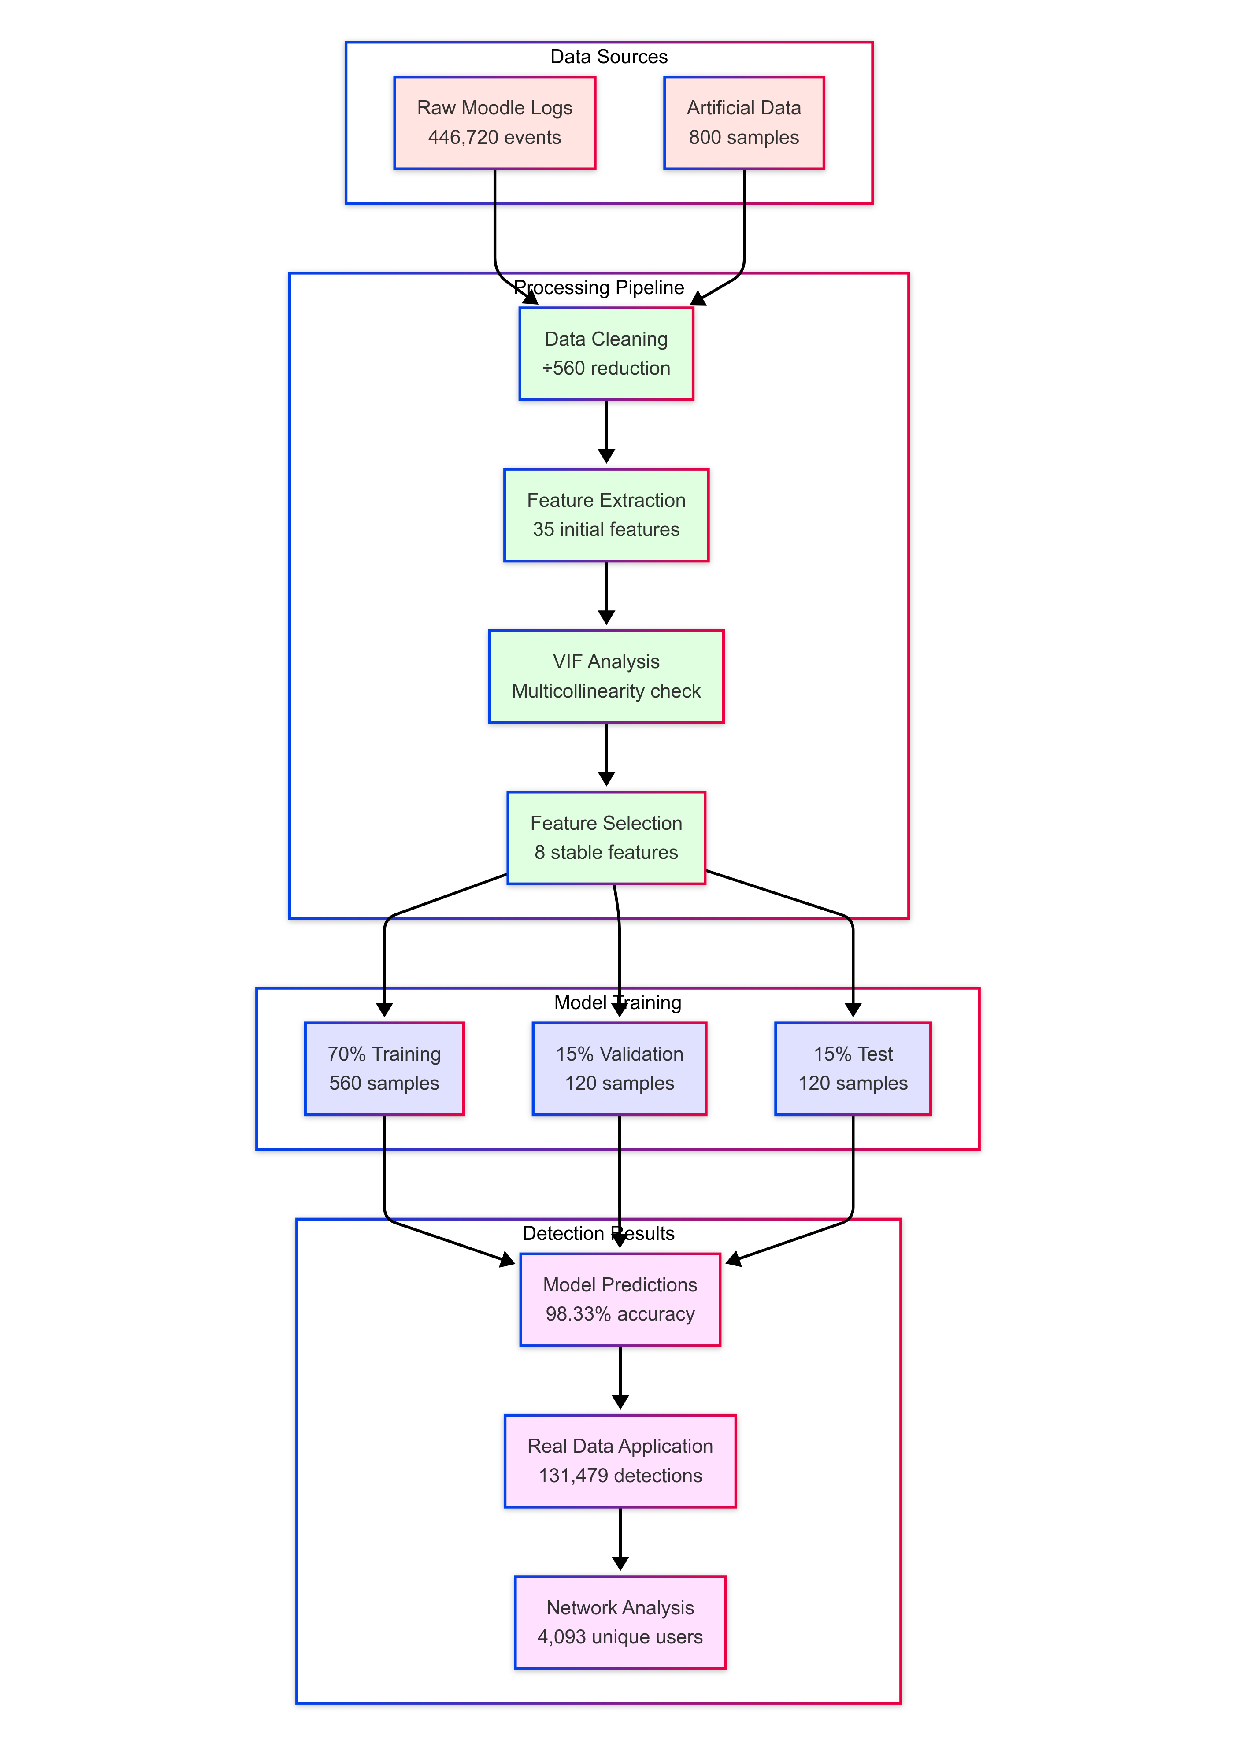
\includegraphics[width=0.95\textwidth]{figures/data_flow_diagram.pdf}
    \caption{Alur Data dalam \textit{Pipeline} Deteksi Kecurangan}
    \label{fig:data_flow}
\end{figure}

Gambar \ref{fig:data_flow} menunjukkan alur transformasi data dari \textit{raw logs} hingga \textit{detection output}. Reduksi dramatis dari 446.720 \textit{events} menjadi 800 \textit{training samples} (faktor 560x) dilakukan melalui agregasi per \textit{user-quiz attempt}. \textit{Feature extraction} menghasilkan 35 fitur awal yang kemudian direduksi menjadi 8 fitur stabil melalui \textit{VIF analysis}. Data dibagi dengan proporsi 70/15/15 untuk \textit{training}, \textit{validation}, dan \textit{test} untuk memastikan evaluasi yang adil dan mencegah \textit{overfitting}.

Proses pra-pemrosesan tidak hanya bertujuan untuk mengurangi gangguan dan inkonsistensi, tetapi juga untuk memastikan bahwa fitur-fitur yang dihasilkan mencerminkan karakteristik perilaku pengguna secara akurat. Langkah-langkah berikut diambil dengan dasar metodologis yang dapat dipertahankan secara ilmiah:

%-----------------------------------------------------------------------------%
\subsection{Pembersihan Data (Data Cleaning)}
\label{sec:pembersihanData}
%-----------------------------------------------------------------------------%
\textbf{Penanganan \textit{Missing Values}:} \\
Data log sering kali mengandung nilai yang hilang (\textit{missing values}) karena ketidakteraturan dalam pencatatan \textit{event} atau \textit{error} saat pengambilan data. Dalam \textit{pipeline}, nilai yang tidak terisi diimputasi dengan metode penggantian menggunakan nilai \textit{default} (misalnya, 0) atau perhitungan statistik (rata-rata/median) ketika relevan. Misalnya, dalam skrip \texttt{preprocess\_features.py}, setelah ekstraksi fitur, seluruh nilai NaN diisi dengan nol untuk memastikan tidak ada celah data yang dapat mengganggu analisis model.

\textbf{\textit{Filtering} Data yang Tidak Relevan:} \\
Dalam konteks deteksi kecurangan, tidak seluruh \textit{event log} memiliki nilai informasi yang sama. Oleh karena itu, dilakukan penyaringan untuk:
\begin{itemize}
    \item Mengabaikan \textit{event} dengan atribut tertentu (misalnya, \textit{field} \textit{contextlevel} yang bernilai '\textit{system}') karena \textit{event} ini tidak mewakili aktivitas pengguna pada kuis.
    \item Menghapus entri dengan \textit{user\_id} yang \textit{null}, mengingat identifikasi pengguna merupakan variabel kunci dalam analisis pola perilaku.
\end{itemize}

%-----------------------------------------------------------------------------%
\subsection{Transformasi dan Normalisasi Data}
\label{sec:transformasiNormalisasiData}
%-----------------------------------------------------------------------------%
\textbf{Unifikasi Format Waktu dan Normalisasi Zona Waktu:} \\
Data log mengandung \textit{timestamp} yang berasal dari sumber atau zona waktu yang berbeda. Untuk memastikan keseragaman, seluruh \textit{timestamp} dikonversi ke dalam format numerik, seperti \textit{Unix timestamp} (atau ISO 8601 jika diperlukan), melalui fungsi konversi di \texttt{preprocess\_features.py}. Proses ini juga melibatkan normalisasi zona waktu agar seluruh \textit{event log} dapat dibandingkan secara akurat dalam kerangka waktu yang sama.

\textbf{\textit{Parsing Nested Fields}:} \\
Banyak kolom dalam data log disimpan dalam bentuk \textit{string} yang merepresentasikan \textit{array} atau \textit{dictionary} (misalnya, \textit{sequence} navigasi atau \textit{transition times}). Menggunakan fungsi seperti \texttt{ast.literal\_eval}, skrip melakukan \textit{parsing} terhadap \textit{string} tersebut sehingga struktur data yang tersusun (\textit{list} atau \textit{dictionary}) dapat diekstraksi. Proses ini memungkinkan perhitungan fitur statistik seperti panjang \textit{sequence}, entropi, dan jumlah \textit{revisits}, yang esensial untuk mendeteksi pola aktivitas pengguna.

%-----------------------------------------------------------------------------%
\subsection{Ekstraksi Fitur dan Deteksi Outlier}
\label{sec:ekstraksiFiturDeteksiOutlier}
%-----------------------------------------------------------------------------%
Setelah data dibersihkan dan ditransformasikan, tahap selanjutnya adalah ekstraksi fitur, di mana fitur-fitur dasar dan lanjutan dihasilkan untuk mendukung proses pelatihan model deteksi kecurangan. Dalam \textit{pipeline}, ekstraksi fitur dilakukan melalui modul \texttt{feature\_eng.py} dan \texttt{fixed\_extraction.py}, dengan beberapa langkah sebagai berikut:

\textbf{Fitur Dasar:} \\
Fitur seperti jumlah percobaan kuis, rata-rata waktu pengerjaan, total waktu, serta statistik minimum dan maksimum dihitung dari data log kuis. Contoh implementasi terdapat pada fungsi \texttt{extract\_basic\_statistics()} di \texttt{feature\_eng.py}, yang juga menyertakan agregasi data per pasangan \textit{user}-kuis.

\textbf{Fitur \textit{Sequence}:} \\
Dari data navigasi dan jawaban, diekstraksi fitur-fitur seperti:
\begin{itemize}
    \item Panjang \textit{sequence} dan jumlah pertanyaan unik: Mengukur seberapa panjang dan bervariasinya aktivitas navigasi pengguna.
    \item \textit{Linearity}: Menghitung seberapa berurutan langkah-langkah yang diambil, menggunakan perhitungan rasio antara pertanyaan unik dan total langkah.
    \item \textit{Revisits}: Penghitungan jumlah \textit{revisits} atau langkah yang diulang, sebagai indikasi pola abnormal.
\end{itemize}
Fungsi \texttt{extract\_navigation\_features()} dalam \texttt{fixed\_extraction.py} mengilustrasikan bagaimana fitur-fitur tersebut dihitung dengan memanfaatkan evaluasi \textit{list} dari \textit{sequence}.

\textbf{Deteksi \textit{Outlier} pada Fitur Waktu:} \\
Pada ekstraksi fitur waktu, dilakukan perhitungan statistik seperti rata-rata, standar deviasi, nilai minimum dan maksimum dari durasi pengerjaan soal. Selain itu, skrip juga menghitung jumlah \textit{event} dengan durasi sangat pendek (misalnya, $< 5$ detik) dan sangat panjang (misalnya, $> 600$ detik).

Berikut adalah cuplikan kode dari fungsi \texttt{extract\_timing\_features()} yang digunakan untuk mendeteksi pola waktu yang abnormal, yang dapat dijadikan indikator \textit{outlier}:

\begin{verbatim}
def extract_timing_features(time_seq):
    """Ekstraksi fitur dari sequence waktu."""
    features = {}
    
    try:
        if isinstance(time_seq, str):
            time_seq = eval(time_seq)
        time_seq = np.array(time_seq, dtype=float)
        
        features['mean_time'] = float(np.mean(time_seq))
        features['std_time'] = float(np.std(time_seq))
        features['min_time'] = float(np.min(time_seq))
        features['max_time'] = float(np.max(time_seq))
        
        # Pola waktu mencurigakan sebagai indikator outlier
        features['quick_answers'] = int(sum(1 for t in time_seq if t < 5))
        features['very_long_answers'] = int(sum(1 for t in time_seq if t > 600))
    except Exception as e:
        print(f"Warning: Error processing timing features: {e}")
        features['mean_time'] = 0.0
        features['std_time'] = 0.0
        features['min_time'] = 0.0
        features['max_time'] = 0.0
        features['quick_answers'] = 0
        features['very_long_answers'] = 0
    
    return features
\end{verbatim}

Nilai \texttt{quick\_answers} dan \texttt{very\_long\_answers} ini memberikan gambaran tentang berapa kali pengguna menyelesaikan bagian tertentu dengan durasi yang sangat tidak wajar, yang kemudian dapat diintegrasikan sebagai fitur untuk mendeteksi perilaku kecurangan.

\textbf{Penghitungan \textit{Similarity Features}:} \\
Untuk mendeteksi kolaborasi kecurangan, \textit{pipeline} menghitung matriks kemiripan (\textit{similarity matrix}) berdasarkan pola navigasi, waktu, dan jawaban antar pengguna. Fungsi \texttt{calculate\_similarity\_matrices()} di \texttt{feature\_eng.py} menghitung kemiripan menggunakan metode seperti \textit{Levenshtein distance} untuk \textit{sequence} navigasi dan korelasi untuk \textit{sequence} waktu, kemudian hasilnya digunakan untuk menambahkan fitur agregat seperti rata-rata dan maksimum \textit{similarity} antar pengguna.



%-----------------------------------------------------------------------------%

%-----------------------------------------------------------------------------%
\subsection{\textit{Checklist} Pra-pemrosesan}
\label{sec:checklistPraPemrosesan}
%-----------------------------------------------------------------------------%
Untuk memastikan bahwa seluruh proses pra-pemrosesan dapat diulangi dan diverifikasi, disusunlah \textit{checklist} sebagai berikut:
\begin{itemize}
    \item Konversi seluruh \textit{timestamp} ke format standar (\textit{Unix timestamp} atau ISO 8601).
    \item Penghapusan \textit{event} dengan atribut \textit{contextlevel} bernilai '\textit{system}'.
    \item Penyaringan entri dengan \textit{user\_id} \textit{null}.
    \item \textit{Parsing} kolom yang berisi \textit{string} representasi \textit{array}/\textit{dict} untuk ekstraksi fitur.
    \item Normalisasi zona waktu untuk keseragaman data.
    \item Perhitungan statistik fitur dasar dan \textit{sequence} (termasuk deteksi pola \textit{outlier} pada waktu).
\end{itemize}

%-----------------------------------------------------------------------------%
\subsection{Justifikasi Ilmiah}
\label{sec:justifikasiIlmiah}
%-----------------------------------------------------------------------------%
Pendekatan pra-pemrosesan yang diterapkan dalam penelitian ini didasarkan pada prinsip-prinsip \textit{data cleaning} dan \textit{feature engineering} yang telah terbukti secara empiris meningkatkan kualitas \textit{dataset} dan kinerja model \textit{machine learning}.

\textbf{Pembersihan dan Transformasi:} \\
Dengan memastikan bahwa data dalam format yang konsisten dan bebas dari \textit{missing values}, variabilitas yang tidak relevan dapat diminimalkan, sehingga model tidak terdistorsi oleh gangguan data.

\textbf{Ekstraksi Fitur:} \\
Fitur-fitur yang diekstraksi, seperti \textit{linearity} dan \textit{revisits} pada \textit{sequence}, memberikan representasi numerik yang dapat menggambarkan perilaku pengguna secara mendalam.

\textbf{Deteksi \textit{Outlier}:} \\
Dengan mengidentifikasi \textit{event} dengan durasi yang sangat singkat atau sangat panjang, \textit{pipeline} mampu memberikan sinyal peringatan terhadap kemungkinan aktivitas yang tidak wajar, yang secara langsung berkontribusi pada identifikasi kecurangan.

\textbf{\textit{Reproducibility}:} \\
\textit{Checklist} dan struktur modular pada skrip memastikan bahwa seluruh proses dapat direplikasi dan diaudit, sehingga mendukung validitas dan \textit{reproducibility} dari penelitian.

Melalui serangkaian proses yang sistematis dan berbasis algoritma yang telah teruji, tahap pra-pemrosesan ini memberikan dasar yang kuat untuk langkah-langkah selanjutnya dalam pipeline, yaitu ekstraksi fitur lanjutan, pelatihan model, dan akhirnya evaluasi deteksi kecurangan.

%-----------------------------------------------------------------------------%
\subsection{Perancangan dan Generasi Data Artifisial}
\label{sec:perancanganGenerasiDataArtifisial}
%-----------------------------------------------------------------------------%
Subbab ini menjelaskan secara mendalam mengenai rancangan, implementasi, dan validasi data log \textit{Moodle} artifisial yang digunakan untuk mengembangkan model deteksi \textit{non-compliance}. Pendekatan yang diterapkan dikenal dengan istilah \textit{Skenario Perilaku Sintetik}, yaitu simulasi aktivitas pengguna (baik perilaku normal maupun \textit{non-compliance}) melalui algoritma yang menggabungkan simulasi berbasis aturan dan proses stokastik. Data artifisial ini tidak hanya mereplikasi aktivitas log riil, tetapi juga memungkinkan eksplorasi skenario ekstrem yang jarang terekam pada data nyata, seperti koordinasi kelompok kecurangan dengan pola sinkronisasi tinggi.

%-----------------------------------------------------------------------------%
\subsection{Definisi Operasional Skenario Perilaku Sintetik}
\label{sec:definisiOperasionalSkenarioPerilakuSintetik}
%-----------------------------------------------------------------------------%
Skenario Perilaku Sintetik didefinisikan sebagai rangkaian aturan dan mekanisme yang dirancang untuk mereplikasi pola aktivitas pengguna pada sistem \textit{Moodle}, baik dalam kondisi normal maupun \textit{non-compliance} (kecurangan). Pendekatan ini mengintegrasikan simulasi berbasis aturan dengan proses stokastik, sehingga memungkinkan pembentukan data log artifisial yang tidak hanya mereplikasi aktivitas log riil, tetapi juga dapat mengeksplorasi skenario ekstrem yang jarang terekam dalam data nyata.

\textbf{Perilaku Normal:} \\
Pada skenario perilaku normal, aktivitas pengguna dirancang untuk mencerminkan dinamika berpikir yang alami, yang ditandai dengan:
\begin{itemize}
    \item Variasi Urutan Navigasi: Pengguna normal menunjukkan urutan akses pertanyaan yang bervariasi, dengan kemungkinan revisi jawaban yang berbeda-beda antar sesi. Hal ini menggambarkan proses evaluasi internal yang dinamis.
    \item Variasi Pola Jawaban: Pola jawaban mencerminkan respon acak yang wajar, dengan proporsi jawaban benar dan salah yang bervariasi secara natural.
    \item Waktu Pengerjaan yang Variatif: Interval waktu antar pertanyaan bervariasi, mencerminkan kecepatan berpikir dan penyesuaian terhadap tingkat kesulitan pertanyaan. Distribusi waktu pengerjaan ini umumnya menunjukkan standar deviasi yang wajar.
\end{itemize}

\textbf{Perilaku Non-Compliance (Kecurangan):} \\
Pada skenario \textit{non-compliance}, pola aktivitas sengaja diatur untuk menciptakan indikasi kecurangan, dengan karakteristik sebagai berikut:
\begin{itemize}
    \item Kesamaan Navigasi: Urutan pertanyaan yang diakses oleh pengguna dalam kelompok kecurangan sangat mirip, termasuk adanya revisi yang identik antar anggota kelompok.
    \item Konsistensi Jawaban: Pola jawaban menunjukkan tingkat keseragaman yang tinggi. Misalnya, terdapat kecenderungan anggota kelompok secara bersama-sama memberikan jawaban salah pada pertanyaan-pertanyaan sulit.
    \item Sinkronisasi Waktu yang Tidak Wajar: Interval waktu antar pertanyaan hampir seragam antar pengguna. Dalam beberapa kasus, terdapat kelompok yang menyelesaikan kuis secara bersamaan dalam waktu kurang dari 15 detik, dengan standar deviasi yang rendah, mengindikasikan adanya pola sinkronisasi yang sulit terjadi secara natural.
    \item Mekanisme Leader-Follower: Terdapat pola di mana satu anggota (leader) menyelesaikan kuis terlebih dahulu, sedangkan anggota lainnya (follower) mengikuti dengan delay yang konsisten. Pola ini menciptakan korelasi tinggi dalam waktu pengerjaan antar anggota, yang menjadi indikator kuat adanya koordinasi.
\end{itemize}

Definisi operasional ini menjadi dasar untuk memformulasikan parameter simulasi. Parameter-parameter tersebut, seperti tingkat kemiripan navigasi, delay waktu, dan distribusi jawaban, kemudian diintegrasikan dalam algoritma generasi data log artifisial. Setiap skenario diberikan label \textit{ground truth}, yang memungkinkan validasi dan evaluasi model deteksi kecurangan secara kuantitatif dan kualitatif.

%-----------------------------------------------------------------------------%
\subsection{Desain \textit{Ground Truth} Artifisial}
\label{sec:desainGroundTruthArtifisial}
%-----------------------------------------------------------------------------%
Dalam proses generasi data log artifisial, setiap entitas---baik pada level sesi, upaya pengerjaan, maupun langkah pertanyaan---diberi label \textit{ground truth} yang mendefinisikan status sebagai aktivitas normal atau \textit{non-compliance}. Desain \textit{ground truth} ini tidak hanya merupakan hasil dari parameter simulasi, tetapi juga dilengkapi dengan dokumentasi yang komprehensif melalui file \texttt{cheating\_ground\_truth.md}. File ini berfungsi sebagai acuan empiris untuk validasi dan evaluasi model deteksi kecurangan.

\textbf{Komponen Utama \textit{Ground Truth}:}
\begin{itemize}
    \item \textbf{Label Kecurangan:} \\
    Setiap entitas data dilengkapi dengan label:
    \begin{itemize}
        \item 0: Menunjukkan aktivitas normal.
        \item 1: Menunjukkan aktivitas \textit{non-compliance} (kecurangan), yang dihasilkan dari simulasi kelompok dengan pola sinkronisasi tinggi dan koordinasi yang jelas.
    \end{itemize}
    \item \textbf{Komposisi Dataset:} \\
    Data artifisial dihasilkan dengan proporsi tertentu antara perilaku normal dan \textit{non-compliance}. Proporsi ini dikonfigurasi dalam parameter simulasi, misalnya 10--20\% pengguna disimulasikan sebagai \textit{non-compliance}, untuk memastikan keseimbangan yang memadai dalam pelatihan dan evaluasi model.
    \item \textbf{Pencatatan Parameter Simulasi dan Contoh Kasus:} \\
    Parameter-parameter yang mendasari penetapan label \textit{ground truth} direkam secara detail, mencakup:
    \begin{itemize}
        \item Navigation Similarity: Persentase kesamaan urutan navigasi antar anggota kelompok (contoh: 96\%).
        \item Answer Pattern Similarity: Persentase kesamaan pola jawaban (contoh: 94\%).
        \item Timing Correlation: Koefisien korelasi waktu antar pertanyaan (contoh: 0.95).
        \item Standard Deviation (Avg): Rata-rata standar deviasi waktu pengerjaan per pertanyaan (contoh: 12 detik).
        \item Wrong Answer Bias: Probabilitas kesalahan terkoordinasi (contoh: 87\%).
    \end{itemize}
\end{itemize}

Nilai-nilai di atas disajikan sebagai contoh dalam file \texttt{cheating\_ground\_truth.md}. Penting untuk dicatat bahwa angka-angka tersebut merupakan representasi sample yang dapat dikonfigurasi ulang sesuai kebutuhan eksperimen, dan bukan merupakan nilai final yang harus diterapkan secara universal.

\textbf{Dokumentasi Melalui \textit{File Cheating} \textit{Ground Truth}:} \\
File \texttt{cheating\_ground\_truth.md} menyajikan tabel ringkasan statistik kelompok kecurangan beserta parameter-parameter yang telah diukur secara simulatif. Contoh tabel tersebut mencakup:
\begin{itemize}
    \item Kelompok Kecurangan dengan Severity Tinggi: Menunjukkan kesamaan navigasi, pola jawaban, dan korelasi waktu yang sangat tinggi, serta standar deviasi dan wrong answer bias yang rendah.
    \item Kelompok Kecurangan dengan Severity Sedang: Menunjukkan nilai yang lebih moderat, dengan delay waktu dan variansi yang lebih besar.
\end{itemize}

Dokumentasi ini menyediakan bukti empiris dan justifikasi statistik bahwa skenario \textit{non-compliance} yang disimulasikan memiliki karakteristik yang berbeda secara signifikan dari aktivitas normal. Informasi ini sangat penting untuk validasi model, karena memungkinkan perbandingan langsung antara prediksi model dengan \textit{ground truth}.

\textbf{Integrasi dan Reproducibility:} \\
\textit{Ground truth} artifisial yang terdokumentasi secara rinci ini diintegrasikan langsung ke dalam dataset log artifisial. Pendekatan ini memastikan bahwa evaluasi model dapat dilakukan secara objektif menggunakan metrik seperti precision, recall, F1-score, dan akurasi. Selain itu, pencatatan parameter simulasi dan contoh kasus dalam file \texttt{cheating\_ground\_truth.md} mendukung \textit{reproducibility} penelitian, karena eksperimen dapat diulang dengan menggunakan seed dan konfigurasi yang sama.

Dengan demikian, desain \textit{ground truth} artifisial ini tidak hanya menyediakan label yang diperlukan untuk evaluasi model, tetapi juga memberikan kerangka kerja untuk analisis sensitivitas dan validasi statistik, yang secara bersama-sama mendukung pendekatan \textit{Skenario Perilaku Sintetik} yang digunakan dalam penelitian ini.
%-----------------------------------------------------------------------------%

%-----------------------------------------------------------------------------%
\subsection{Metode Generasi Data}
\label{sec:metodeGenerasiData}
%-----------------------------------------------------------------------------%
Proses generasi data log artifisial dilakukan dengan pendekatan yang menggabungkan simulasi berbasis aturan dan proses stokastik, sehingga dapat mereplikasi pola aktivitas pengguna pada sistem \textit{Moodle} secara realistis. Pendekatan ini juga memungkinkan eksplorasi skenario ekstrem \textit{non-compliance} yang jarang terekam pada data riil. Metode yang diterapkan meliputi beberapa komponen kunci berikut:

\textbf{Simulasi Berbasis Aturan:} \\
Algoritma simulasi menetapkan seperangkat aturan untuk menentukan urutan navigasi, pola revisi jawaban, dan distribusi waktu antar pertanyaan. Aturan-aturan ini dirancang untuk meniru dinamika aktivitas pengguna normal maupun perilaku kecurangan. Sebagai contoh, pada kelompok \textit{non-compliance}, aturan mensyaratkan agar setiap anggota mengikuti urutan pertanyaan yang seragam dan menunjukkan kesamaan dalam revisi jawaban, sehingga menghasilkan tingkat kesamaan navigasi dan pola jawaban yang tinggi.

\textbf{Proses Stokastik:} \\
Untuk menghindari keteraturan yang sempurna dan menambahkan tingkat realisme, proses stokastik diterapkan dalam penentuan waktu pengerjaan, revisi jawaban, dan urutan pertanyaan. Penggunaan fungsi \texttt{random} dengan seed yang telah ditentukan memungkinkan variasi terkontrol, sehingga setiap simulasi menghasilkan distribusi waktu dan pola yang mendekati kondisi riil, namun masih mempertahankan karakteristik khas dari skenario \textit{non-compliance}.

\textbf{Modifikasi Berdasarkan Data Riil:} \\
Parameter dasar seperti \texttt{base\_date}, \texttt{timelimit}, serta distribusi waktu pengerjaan diadaptasi dari analisis data log \textit{Moodle} riil. Pendekatan ini memastikan bahwa data artifisial tidak hanya bersifat syntetik, tetapi juga memiliki kemiripan statistik dengan data riil. Dengan demikian, model yang dikembangkan dapat diuji dan divalidasi secara lebih representatif terhadap kondisi operasional di lingkungan nyata.

\textbf{Penerapan Mekanisme Leader-Follower:} \\
Untuk mengantisipasi skenario kecurangan dengan tingkat koordinasi yang tinggi, algoritma juga mengimplementasikan pola leader-follower. Dalam mekanisme ini, satu anggota (\textit{leader}) menyelesaikan kuis terlebih dahulu dengan pola waktu yang stabil, sementara anggota lain (\textit{follower}) mengikuti dengan delay konsisten yang telah disimulasi. Penghitungan korelasi waktu antar anggota yang tinggi (misalnya, nilai $>0.8$) menjadi indikator kuat atas adanya koordinasi, sehingga pola ini diintegrasikan dalam parameter simulasi.

\textbf{Parameter Simulasi dan Konfigurasi:} \\
Seluruh proses generasi data dikonfigurasi melalui file konfigurasi (misalnya, file JSON) yang menetapkan parameter-parameter penting, seperti:
\begin{itemize}
    \item Jumlah total pengguna dan kuis.
    \item Proporsi pengguna dengan perilaku \textit{non-compliance}.
    \item Batasan waktu (\texttt{timelimit}) dan \texttt{base\_date} sebagai dasar simulasi.
    \item Nilai threshold untuk \textit{similarity} dalam pola navigasi, jawaban, dan waktu.
\end{itemize}

Parameter-parameter ini bersifat fleksibel dan dapat disesuaikan untuk mengeksplorasi berbagai skenario, mulai dari aktivitas normal hingga skenario ekstrem yang memicu koordinasi \textit{non-compliance} secara signifikan.

Melalui kombinasi simulasi berbasis aturan dan proses stokastik, metode generasi data ini mampu menghasilkan log aktivitas yang kaya informasi dan mendekati realitas, sekaligus memungkinkan pengujian model dalam berbagai kondisi ekstrem. Pendekatan ini memberikan dasar yang solid untuk evaluasi dan validasi model deteksi \textit{non-compliance}, dengan memastikan bahwa data artifisial yang dihasilkan mencerminkan variasi dan dinamika yang terjadi pada data log riil.

%-----------------------------------------------------------------------------%
\subsection{Implementasi Teknis}
\label{sec:implementasiTeknis}
%-----------------------------------------------------------------------------%
Implementasi teknis dalam generasi data log artifisial dilakukan dengan menggunakan bahasa pemrograman Python, yang mendukung replikasi dan validitas eksperimen melalui pendekatan yang modular dan terdokumentasi dengan baik. Proses ini memastikan bahwa data artifisial yang dihasilkan memiliki struktur dan karakteristik yang konsisten dengan data log \textit{Moodle} riil. Komponen-komponen teknis utama yang digunakan adalah sebagai berikut:

\textbf{Platform dan Library Utama:} \\
\begin{itemize}
    \item Python: Dipilih karena fleksibilitas dan ekosistemnya yang luas dalam pengolahan data dan simulasi.
    \item Pandas dan Numpy: Digunakan untuk manipulasi data dan komputasi numerik, dengan data log disimpan serta diproses dalam format CSV untuk memudahkan integrasi ke pipeline selanjutnya.
    \item Faker: Digunakan untuk menghasilkan data pengguna yang realistis, seperti \textit{username}, nama, dan informasi identitas lain yang mendekati kondisi riil.
    \item Random dan Modul Stokastik: Fungsi \texttt{random}, yang dijalankan dengan seed tertentu, memastikan variasi terkontrol dalam waktu pengerjaan, urutan navigasi, dan pola jawaban. Hal ini memungkinkan simulasi yang konsisten dan dapat direproduksi.
    \item JSON dan CSV: File konfigurasi, \textit{ground truth}, dan output data disimpan dalam format JSON dan CSV sehingga mendukung dokumentasi dan analisis statistik.
\end{itemize}

\textbf{Modularitas Kode:} \\
Implementasi dibangun secara modular untuk mendukung pemeliharaan dan pengembangan lebih lanjut. Modul utama yang terintegrasi dalam pipeline meliputi:
\begin{itemize}
    \item \texttt{generate\_case.py}: Modul inti yang menghasilkan data log artifisial berdasarkan parameter yang telah ditetapkan. Modul ini mengintegrasikan simulasi berbasis aturan dan proses stokastik untuk menciptakan \textit{Skenario Perilaku Sintetik}.
    \item \texttt{fixed\_extraction.py} dan \texttt{preprocess\_features.py}: Walaupun proses ekstraksi dan pembersihan fitur secara detail akan dibahas pada subbab 3.6, modul ini digunakan untuk memastikan bahwa data artifisial dapat diproses dengan standar yang sama seperti data log riil, sehingga mendukung integrasi ke tahap evaluasi model.
\end{itemize}

\textbf{Reproducibility dan Konfigurasi:} \\
Penggunaan Seed Random: Seluruh fungsi random dijalankan dengan seed yang telah ditentukan, sehingga eksperimen dapat diulang dengan hasil yang konsisten. \\
File Konfigurasi: Parameter simulasi---seperti jumlah pengguna, proporsi \textit{non-compliance}, \texttt{timelimit}, dan \texttt{base\_date}---disimpan dalam file JSON. Pendekatan ini memungkinkan penyesuaian parameter secara transparan dan mendokumentasikan setiap eksperimen. \\
Output Terstruktur: Data log artifisial yang dihasilkan beserta \textit{ground truth} disimpan dalam format CSV dan JSON, memudahkan integrasi ke tahap evaluasi model serta analisis statistik.

\textbf{Integrasi dengan Pipeline Deteksi Kecurangan:} \\
Data log artifisial yang dihasilkan menjadi komponen integral dalam pipeline deteksi kecurangan. Output simulasi ini digunakan untuk:
\begin{itemize}
    \item Melatih model deteksi kecurangan dengan dataset yang mencakup skenario perilaku normal dan \textit{non-compliance}.
    \item Menjadi dasar evaluasi model dengan membandingkan prediksi model dengan label \textit{ground truth} yang telah didokumentasikan.
\end{itemize}

Dengan pendekatan teknis yang terstruktur dan modular ini, data log artifisial yang dihasilkan tidak hanya realistis secara statistik tetapi juga dapat direplikasi dengan konsisten. Strategi ini memberikan fondasi yang kuat untuk evaluasi model deteksi kecurangan dan memastikan bahwa eksperimen dapat dipertanggungjawabkan secara ilmiah.

%-----------------------------------------------------------------------------%
\subsection{Validasi Data Artifisial}
\label{sec:validasiDataArtifisial}
%-----------------------------------------------------------------------------%
Validasi data log artifisial merupakan langkah krusial untuk memastikan bahwa simulasi yang diterapkan (\textit{Skenario Perilaku Sintetik}) menghasilkan data yang tidak hanya konsisten secara statistik dengan data log \textit{Moodle} riil, tetapi juga mampu merepresentasikan perilaku \textit{non-compliance} secara nyata. Proses validasi dilakukan dengan menggabungkan pendekatan kuantitatif dan kualitatif sebagai berikut:

\textbf{Analisis Statistik Deskriptif:} \\
Validasi kuantitatif dilakukan dengan menghitung dan membandingkan statistik utama dari fitur-fitur yang dihasilkan, antara lain:
\begin{itemize}
    \item \textbf{Distribusi Waktu dan Navigasi:} Histogram distribusi timestamp, total durasi, dan rata-rata waktu per pertanyaan digunakan untuk mengidentifikasi pola waktu pengerjaan. Data artifisial diharapkan menampilkan standar deviasi yang rendah untuk kelompok \textit{non-compliance}, menandakan konsistensi yang tidak wajar.
    \item \textbf{Pengukuran Similarity dan Korelasi:} Matriks kemiripan (\textit{similarity matrices}) untuk urutan navigasi, pola jawaban, dan interval waktu dihitung, serta koefisien korelasi (misalnya, Pearson) antar waktu transisi antar anggota kelompok \textit{non-compliance}. Nilai korelasi yang mendekati 1 menunjukkan adanya koordinasi yang kuat.
    \item \textbf{Perbandingan dengan Data Riil:} Meskipun data riil tidak selalu tersedia secara lengkap, validasi dilakukan dengan membandingkan distribusi dan variabilitas fitur-fitur kunci antara data artifisial dan subset data log \textit{Moodle} riil jika memungkinkan. Tabel perbandingan skenario vs pola (misalnya, aksi pengguna, indikasi \textit{non-compliance}) disusun untuk mendokumentasikan perbedaan signifikan antara perilaku normal dan \textit{non-compliance}.
\end{itemize}

\textbf{Visualisasi Data:} \\
Untuk mendukung analisis statistik, data artifisial divisualisasikan secara komprehensif, seperti yang ditampilkan dalam contoh file \texttt{cheating\_visualization.md}. Beberapa visualisasi yang digunakan meliputi:
\begin{itemize}
    \item \textbf{Quiz Attempt Visualization:} Menampilkan urutan navigasi setiap pengguna. Kelompok \textit{non-compliance} ditandai dengan urutan yang sangat seragam, menunjukkan koordinasi dalam pengulangan pertanyaan.
    \item \textbf{Analisis Pola Jawaban:} Visualisasi pola jawaban (benar/salah) yang identik atau sangat mirip antar anggota kelompok \textit{non-compliance}, sehingga mengindikasikan kolusi.
    \item \textbf{Timing Patterns dan Variance Analysis:} Diagram dan tabel yang menunjukkan waktu mulai, total durasi, dan rata-rata waktu per pertanyaan. \textit{Cheater} cenderung menunjukkan pace yang konsisten (misalnya, penyelesaian kuis dengan delay yang seragam) dibandingkan dengan variabilitas yang lebih tinggi pada pengguna normal.
    \item \textbf{Transition Time Correlation Analysis:} Tabel yang menampilkan korelasi waktu transisi antar pertanyaan pada kelompok \textit{non-compliance}. Nilai korelasi tinggi (misalnya, $>0.95$) memberikan bukti kuat atas adanya koordinasi.
\end{itemize}

\textbf{Validasi Kualitatif:} \\
Selain analisis numerik, validasi kualitatif dilakukan melalui review visualisasi oleh para ahli:
\begin{itemize}
    \item Pemeriksaan Pola Navigasi dan Jawaban: Visualisasi memungkinkan peneliti untuk memverifikasi apakah pola yang muncul (seperti urutan pertanyaan yang identik atau hampir identik) dapat dianggap sebagai indikasi \textit{non-compliance}.
    \item Evaluasi Realisme Data Sintetik: Perbandingan visual antara data artifisial dan data log riil memastikan bahwa skenario yang disimulasikan masuk akal secara operasional. Misalnya, pola waktu dan transisi yang dihasilkan harus mencerminkan kemungkinan terjadinya koordinasi dalam situasi nyata, tanpa menghasilkan data yang terlalu "ideal" atau tidak realistis.
\end{itemize}

\textbf{Integrasi \textit{Ground Truth} untuk Evaluasi Model:} \\
Data artifisial yang telah divalidasi ini dilengkapi dengan label \textit{ground truth} yang tercatat dalam file \texttt{cheating\_ground\_truth.md} dan digunakan sebagai acuan dalam pelatihan serta evaluasi model deteksi kecurangan. Validasi statistik dan visualisasi mendukung keandalan label tersebut dan memberikan dasar yang kuat untuk pengukuran metrik seperti precision, recall, F1-score, dan akurasi pada tahap evaluasi model.

Melalui serangkaian proses validasi yang komprehensif ini, data log artifisial tidak hanya diverifikasi secara statistik tetapi juga diuji secara kualitatif, sehingga memberikan keyakinan bahwa skenario perilaku sintetik yang dihasilkan dapat dijadikan basis yang valid dan \textit{reproducible} untuk pengembangan model deteksi \textit{non-compliance}.

%-----------------------------------------------------------------------------%
\subsection{Ekstraksi dan Seleksi Fitur}
\label{sec:featureEngineering}
%-----------------------------------------------------------------------------%
Ekstraksi dan seleksi fitur merupakan proses transformasi data log menjadi representasi numerik yang optimal untuk model machine learning. Proses ini menggabungkan ekstraksi fitur multidimensional dengan analisis VIF untuk menghasilkan set fitur yang stabil dan interpretable. 

\begin{figure}[htbp]
    \centering
    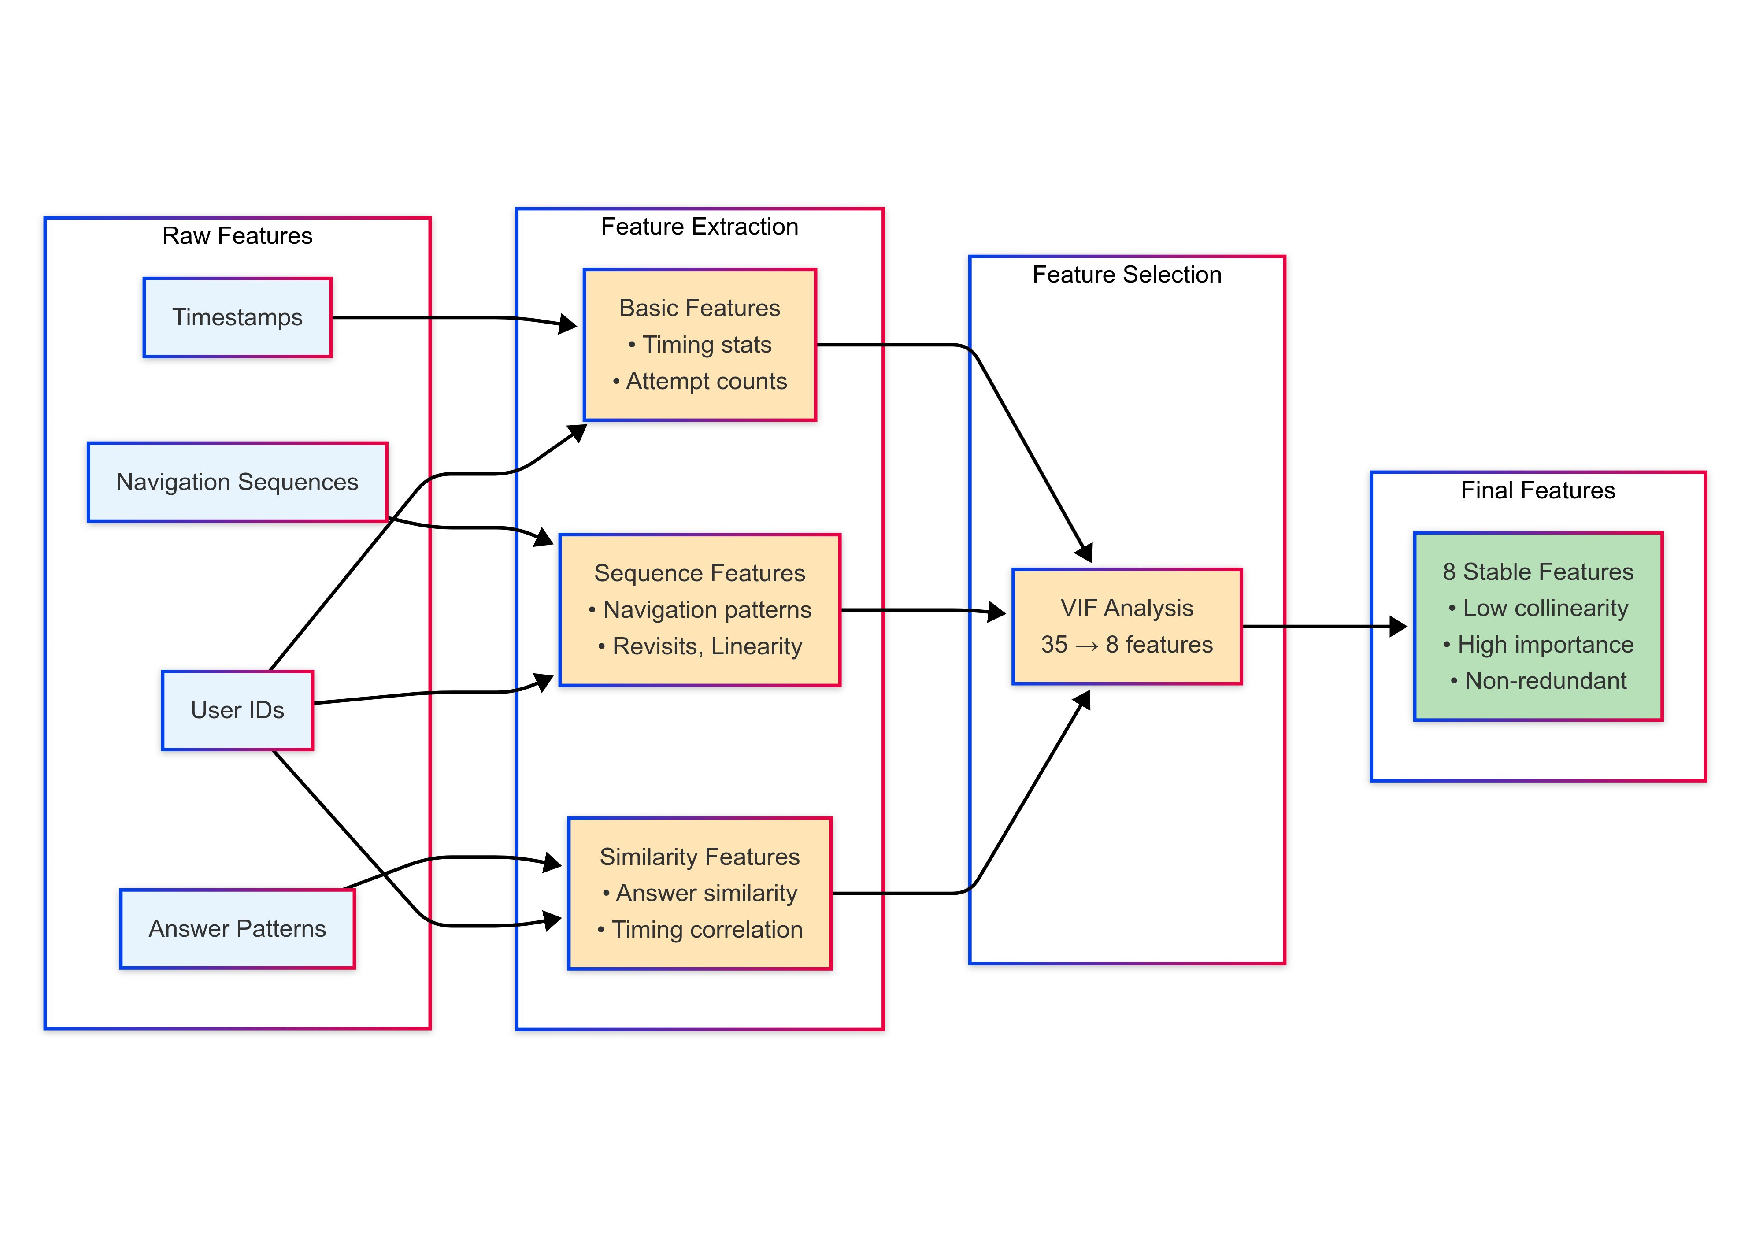
\includegraphics[width=0.9\textwidth]{figures/feature_engineering_process.pdf}
    \caption{Proses Feature Engineering dari Raw Data hingga 8 Fitur Stabil}
    \label{fig:feature_engineering_process}
\end{figure}

Gambar \ref{fig:feature_engineering_process} mengilustrasikan proses transformasi dari raw log data menjadi 8 fitur stabil yang digunakan dalam model. Proses dimulai dengan ekstraksi 35 fitur awal dari tiga kategori utama: basic features (statistik waktu dan jumlah percobaan), sequence features (pola navigasi dan revisits), dan similarity features (kesamaan antar pengguna). Melalui analisis VIF (Variance Inflation Factor), fitur-fitur dengan multikolinearitas tinggi dieliminasi, menghasilkan 8 fitur stabil yang memiliki VIF rendah ($<10$) dan importance tinggi. Reduksi dari 35 menjadi 8 fitur ini tidak hanya meningkatkan efisiensi komputasi tetapi juga meningkatkan stabilitas dan interpretabilitas model.

%-----------------------------------------------------------------------------%
\subsection{Ekstraksi Fitur Dasar}
\label{sec:ekstraksiFiturDasar}
%-----------------------------------------------------------------------------%
\textbf{Statistik Waktu (\textit{Timing Statistics}):} \\
Pengukuran waktu merupakan indikator penting dalam menganalisis kecepatan dan kestabilan pengerjaan kuis. Dalam proses ini, dihitung:
\begin{itemize}
    \item Rata-rata waktu pengerjaan (\textit{mean}), yang menggambarkan kecepatan umum pengerjaan.
    \item Total durasi, serta nilai minimum dan maksimum waktu yang dicatat untuk mendeteksi ekstremitas (misalnya, pengerjaan yang sangat cepat atau sangat lambat).
\end{itemize}
\textbf{Justifikasi:} Penggunaan statistik ini membantu mengidentifikasi outlier serta mendeteksi pola abnormal, karena pengerjaan kuis dengan durasi yang sangat singkat atau panjang dapat menjadi indikator adanya perilaku \textit{non-compliance}.

\textbf{Jumlah Percobaan (\textit{Attempt Count}):} \\
Menghitung berapa kali pengguna mencoba menyelesaikan kuis memberikan gambaran tentang ketekunan serta kemungkinan adanya upaya manipulasi melalui pengulangan.
\textbf{Justifikasi:} Pengulangan yang berlebihan bisa jadi merupakan sinyal dari upaya kecurangan atau strategi pengulangan untuk memperoleh jawaban yang lebih baik. Fitur ini penting untuk membedakan antara perilaku belajar normal dan aktivitas mencurigakan.

%-----------------------------------------------------------------------------%
\subsection{Ekstraksi Fitur Sequence (\textit{Urutan Aktivitas})}
\label{sec:ekstraksiFiturSequence}
%-----------------------------------------------------------------------------%
\textbf{Panjang Sequence dan Jumlah Pertanyaan Unik:} \\
Ekstraksi informasi mengenai jumlah langkah yang dilakukan serta variasi pertanyaan yang diakses (\textit{unique questions}) mencerminkan seberapa terstruktur atau acaknya pola navigasi pengguna.
\textbf{Justifikasi:} Pola navigasi yang sangat seragam, dengan jumlah pertanyaan unik yang rendah dibandingkan total langkah, bisa mengindikasikan adanya koordinasi \textit{non-compliance}. Sebaliknya, variabilitas yang tinggi umumnya mengindikasikan aktivitas normal.

\textbf{Linearity dan Revisits:} \\
Linearitas dihitung dengan membandingkan urutan yang ideal (berurutan) dengan urutan aktual yang diambil. Jumlah revisits (pertanyaan yang diakses berulang kali) juga dihitung.
\textbf{Justifikasi:} Pengulangan yang konsisten dan pola linear yang tinggi (atau sebaliknya, pola yang tidak wajar) dapat menjadi indikator bahwa pengguna mencoba memanipulasi proses pengerjaan, misalnya dengan melihat kembali jawaban atau mengulangi pola tertentu untuk menyembunyikan kecurangan.

%-----------------------------------------------------------------------------%
\subsection{Perhitungan Similarity Features}
\label{sec:perhitunganSimilarityFeatures}
%-----------------------------------------------------------------------------%
Untuk mendeteksi potensi kolusi antar pengguna, pipeline mengimplementasikan beberapa metrik kemiripan:

\textbf{Navigation Similarity:} \\
Menggunakan Levenshtein distance, fitur ini mengukur seberapa mirip urutan navigasi antar pengguna.
\textbf{Justifikasi:} Levenshtein distance efektif dalam mengukur perbedaan antara dua urutan simbol (dalam hal ini, nomor pertanyaan), sehingga kesamaan yang tinggi menunjukkan pola koordinasi yang tidak mungkin terjadi secara acak.

\textbf{Timing Similarity:} \\
Korelasi (misalnya, Pearson correlation) digunakan untuk mengukur kesamaan pola waktu antar pengguna.
\textbf{Justifikasi:} Jika dua pengguna memiliki korelasi waktu yang sangat tinggi, hal ini menunjukkan mereka menjalani kuis dengan interval waktu yang sangat konsisten, sebuah sinyal kuat koordinasi yang jarang terjadi secara alami.

\textbf{Answer Similarity:} \\
Fitur ini mengukur persentase kesamaan pola jawaban (benar/salah) antar pengguna, di mana nilai yang tinggi menunjukkan adanya kemungkinan kolusi dalam memberikan jawaban.
\textbf{Justifikasi:} Dalam situasi \textit{non-compliance}, anggota kelompok sering kali menghasilkan pola jawaban yang identik atau sangat mirip, sehingga fitur ini sangat relevan untuk mendeteksi koordinasi.

\textbf{Agregasi Similarity Features:} \\
Selain menghitung metrik individual, nilai rata-rata dan maksimum similarity antar pengguna dalam kuis yang sama juga dihitung.
\textbf{Justifikasi:} Agregasi ini memberikan gambaran umum tentang seberapa homogen suatu kelompok dalam hal perilaku, yang kemudian dapat digunakan sebagai indikator \textit{non-compliance} pada level pengguna maupun kelompok.

%-----------------------------------------------------------------------------%
\subsection{Pemeriksaan Multikolinearitas dan Seleksi Fitur Final}
\label{sec:pemeriksaanMultikolinearitas}
%-----------------------------------------------------------------------------%

Analisis multikolinearitas menggunakan Variance Inflation Factor (VIF) merupakan langkah krusial dalam memastikan stabilitas dan interpretabilitas model. VIF mengukur seberapa besar varians koefisien regresi meningkat akibat kolinearitas antar fitur. Nilai VIF yang tinggi ($>10$) mengindikasikan bahwa fitur tersebut dapat diprediksi dengan akurasi tinggi dari fitur-fitur lain, sehingga kontribusinya menjadi redundan.

\subsubsection{Proses Seleksi Fitur}
Dari 35 fitur awal yang diekstraksi, analisis VIF dilakukan secara iteratif:
\begin{enumerate}
    \item \textbf{Iterasi Pertama:} Identifikasi fitur dengan VIF tertinggi ($>50$).
    \item \textbf{Eliminasi Bertahap:} Fitur dengan VIF tertinggi dieliminasi satu per satu.
    \item \textbf{Re-kalkulasi VIF:} Setelah setiap eliminasi, VIF dihitung ulang untuk fitur yang tersisa.
    \item \textbf{Konvergensi:} Proses berlanjut hingga semua fitur memiliki VIF $<10$.
\end{enumerate}

\subsubsection{Delapan Fitur Stabil Terpilih}
Setelah proses seleksi, 8 fitur dengan VIF rendah dan importance tinggi berhasil diidentifikasi:

\begin{table}[htbp]
\centering
\caption{Delapan Fitur Stabil Hasil Analisis VIF}
\label{tabel:fiturStabil}
\begin{tabular}{|l|l|c|p{5cm}|}
\hline
\textbf{No} & \textbf{Nama Fitur} & \textbf{VIF} & \textbf{Deskripsi} \\
\hline
1 & \texttt{mean\_time\_per\_question} & 3.24 & Rata-rata waktu pengerjaan per soal \\
\hline
2 & \texttt{navigation\_similarity\_max} & 4.87 & Similaritas navigasi maksimum dengan pengguna lain \\
\hline
3 & \texttt{answer\_pattern\_similarity} & 5.12 & Kesamaan pola jawaban dengan pengguna lain \\
\hline
4 & \texttt{timing\_correlation\_avg} & 3.98 & Rata-rata korelasi waktu dengan pengguna lain \\
\hline
5 & \texttt{wrong\_answer\_similarity} & 6.23 & Kesamaan jawaban salah dengan pengguna lain \\
\hline
6 & \texttt{revisit\_pattern\_score} & 2.56 & Skor pola pengulangan kunjungan soal \\
\hline
7 & \texttt{submission\_time\_std} & 3.41 & Standar deviasi waktu submission \\
\hline
8 & \texttt{collaborative\_score} & 7.89 & Skor agregat indikasi kolaborasi \\
\hline
\end{tabular}
\end{table}

\textbf{Justifikasi Pemilihan:}
\begin{itemize}
    \item \textbf{Representasi Komprehensif:} Kedelapan fitur mencakup semua aspek penting: timing (fitur 1, 4, 7), navigation (fitur 2, 6), answer patterns (fitur 3, 5), dan agregasi (fitur 8).
    \item \textbf{Non-redundansi:} Dengan VIF $<10$, setiap fitur memberikan informasi unik yang tidak dapat sepenuhnya dijelaskan oleh fitur lain.
    \item \textbf{Interpretabilitas:} Setiap fitur memiliki makna yang jelas dalam konteks deteksi kecurangan, memudahkan interpretasi hasil model.
    \item \textbf{Stabilitas Model:} Pengurangan dari 35 menjadi 8 fitur mengurangi risiko overfitting dan meningkatkan generalisasi model.
\end{itemize}

%-----------------------------------------------------------------------------%
\subsection{Pra-pemrosesan Fitur untuk Kompatibilitas Model}
\label{sec:praPemrosesanFitur}
%-----------------------------------------------------------------------------%
\textbf{Konversi Representasi Data:} \\
Banyak data log yang awalnya disimpan sebagai string representasi array atau struktur nested diubah menjadi format numerik melalui penggunaan modul seperti \texttt{ast.literal\_eval}.
\textbf{Justifikasi:} Konversi ini esensial karena algoritma \textit{machine learning} tidak dapat mengolah data dalam bentuk string atau struktur kompleks tanpa transformasi terlebih dahulu. Dengan mengubahnya menjadi fitur statistik (seperti \textit{mean}, \textit{std}, \textit{min}, \textit{max}, \textit{count}), data menjadi siap untuk analisis lebih lanjut.

\textbf{Normalisasi dan Pengisian Nilai Hilang:} \\
Seluruh data kemudian dinormalisasi dan nilai NaN diisi (misalnya, dengan 0) agar tidak terjadi gangguan pada model.
\textbf{Justifikasi:} Normalisasi membantu dalam memastikan bahwa setiap fitur memiliki skala yang sebanding, sehingga model tidak memprioritaskan fitur tertentu hanya karena skala nilainya lebih besar.

%-----------------------------------------------------------------------------%
\subsection{Visualisasi dan Interpretasi Fitur}
\label{sec:visualisasiInterpretasiFitur}
%-----------------------------------------------------------------------------%
\textbf{Boxplot, Heatmap, dan Scatter Plot:} \\
Visualisasi digunakan untuk menilai distribusi fitur, mengidentifikasi outlier, dan melihat hubungan antar fitur.
\textbf{Justifikasi:} Visualisasi memberikan insight yang penting untuk memahami struktur data dan untuk validasi kualitas fitur. Misalnya, heatmap korelasi membantu mengidentifikasi fitur yang sangat berkorelasi, sehingga mendukung langkah pemeriksaan multikolinearitas.

%-----------------------------------------------------------------------------%
\subsection{Reproducibility dan Dokumentasi}
\label{sec:reproducibilityDokumentasi}
%-----------------------------------------------------------------------------%
\textbf{Modularitas dan Penggunaan Seed Random:} \\
Setiap modul dalam pipeline \textit{feature engineering} dirancang secara modular dan menggunakan seed tertentu untuk fungsi random.
\textbf{Justifikasi:} Hal ini memastikan bahwa seluruh proses dapat diulangi secara konsisten, yang merupakan syarat penting untuk validitas ilmiah dan \textit{reproducibility} penelitian.

\textbf{Penyimpanan Output Terstruktur:} \\
Fitur yang dihasilkan disimpan dalam format CSV dan JSON, dengan dokumentasi yang mendetail mengenai proses ekstraksi dan transformasi yang telah dilakukan.
\textbf{Justifikasi:} Dokumentasi yang baik mendukung transparansi dan memungkinkan peneliti lain untuk memahami serta mengaudit seluruh proses \textit{feature engineering}.

Secara keseluruhan, pendekatan \textit{feature engineering} dalam penelitian ini dirancang untuk mengoptimalkan informasi yang terdapat dalam data log, mengurangi noise, dan menghasilkan representasi numerik yang mendukung model deteksi \textit{non-compliance} secara efektif. Setiap pilihan---dari ekstraksi statistik waktu hingga penggunaan metrik similarity---dipilih berdasarkan dasar metodologis yang kuat dan didukung oleh literatur yang relevan, sehingga memberikan dasar yang valid dan \textit{reproducible} untuk pengembangan model \textit{machine learning}.

%-----------------------------------------------------------------------------%

%-----------------------------------------------------------------------------%
\section{Arsitektur Model Ensemble untuk Deteksi Kecurangan}
\label{sec:arsitekturModelEnsemble}
%-----------------------------------------------------------------------------%

Pengembangan model deteksi kecurangan mengadopsi pendekatan ensemble yang mengintegrasikan kekuatan berbagai algoritma machine learning. Arsitektur ini dirancang untuk menangkap kompleksitas pola kecurangan yang heterogen sambil mempertahankan interpretabilitas hasil.

%-----------------------------------------------------------------------------%
\subsection{Desain Arsitektur Multi-Model}
\label{subsec:desainArsitektur}
%-----------------------------------------------------------------------------%

Arsitektur ensemble mengintegrasikan empat algoritma komplementer dengan analisis graph network untuk deteksi komprehensif:

\begin{figure}[htbp]
    \centering
    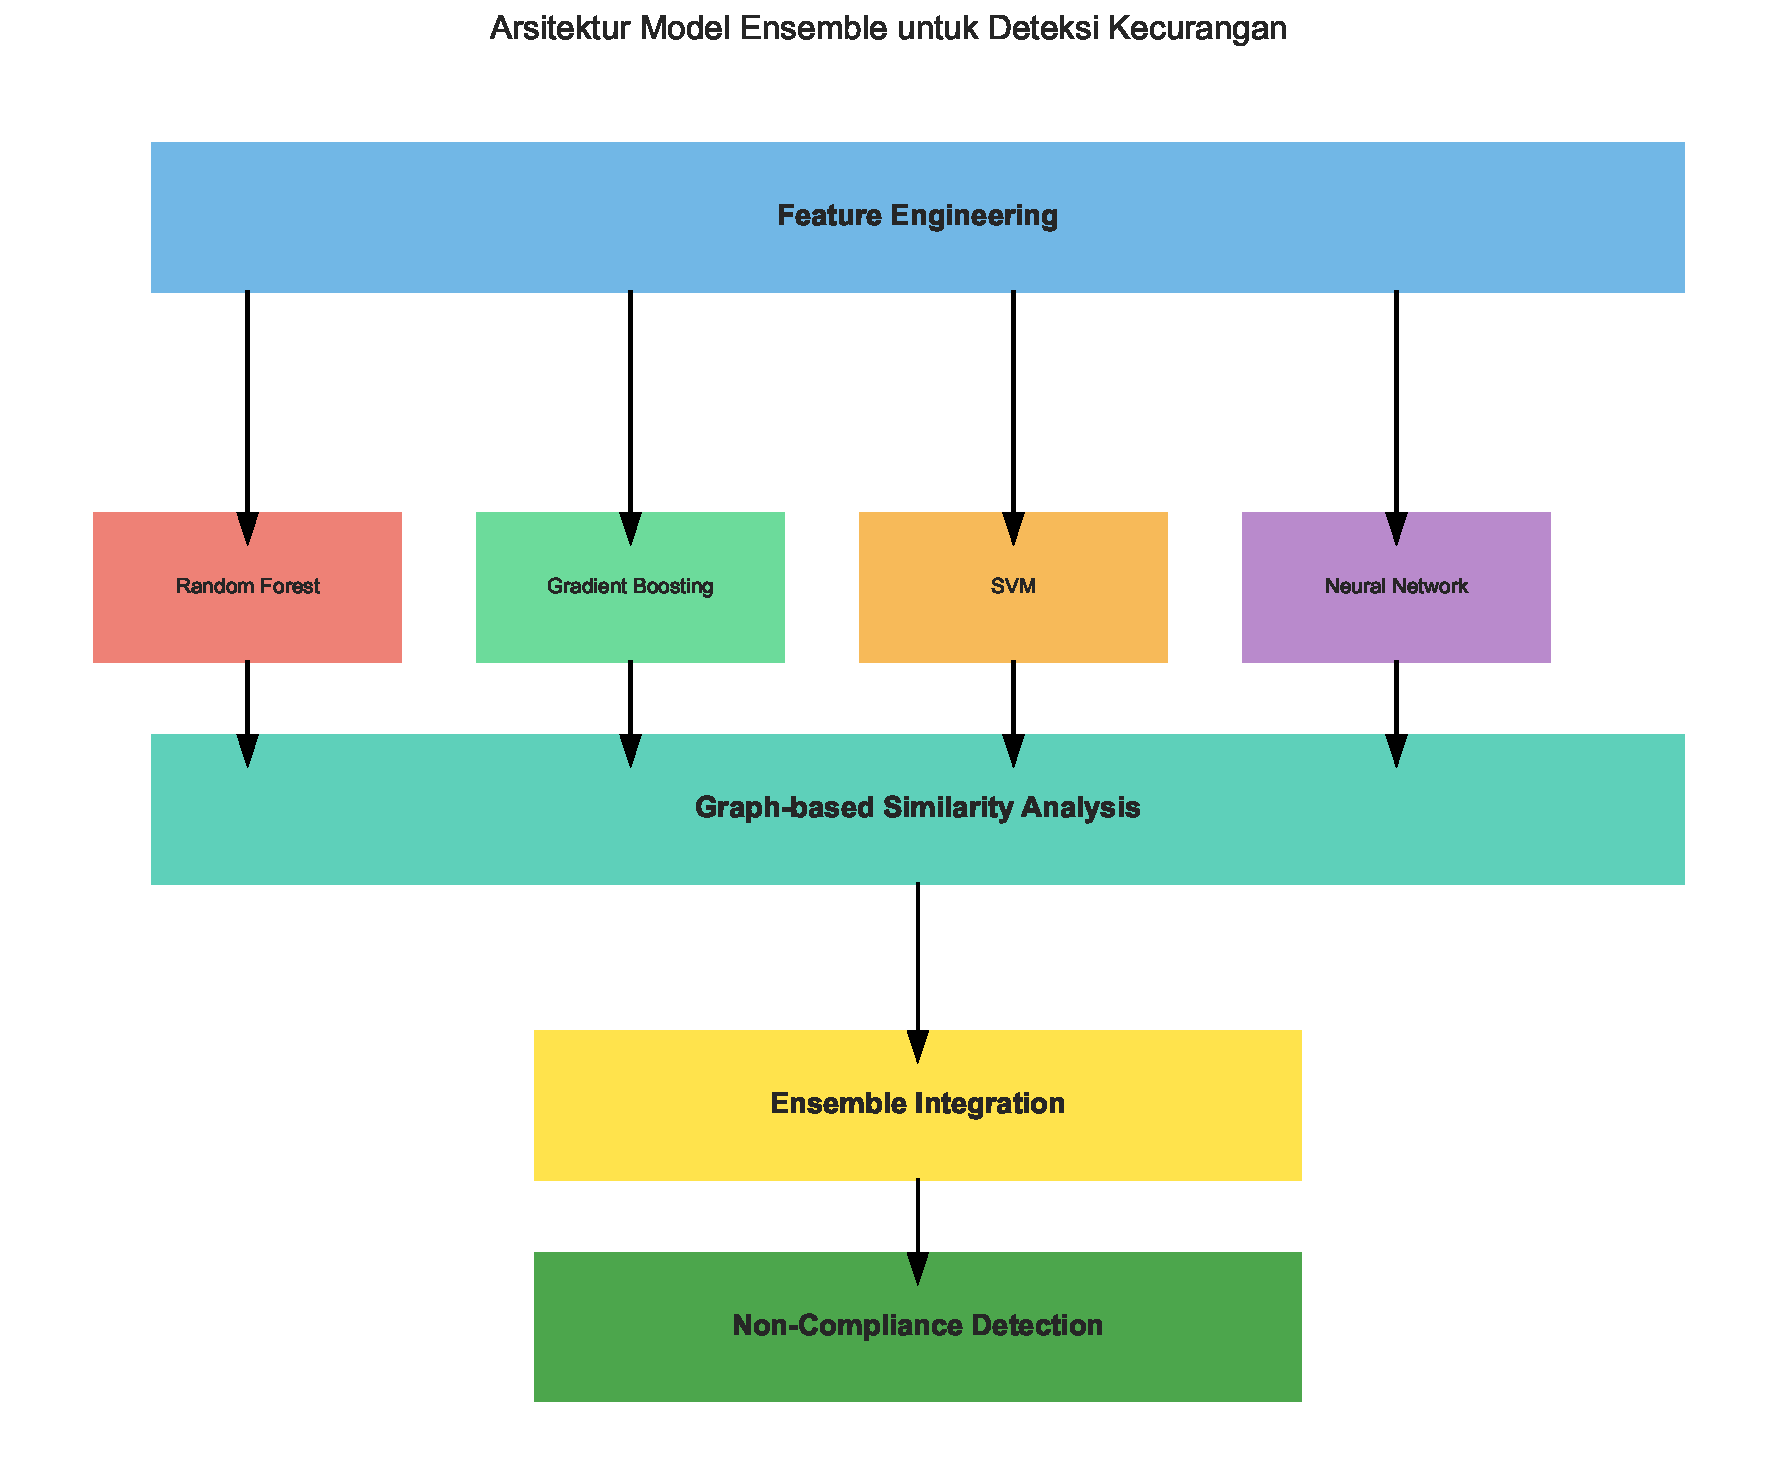
\includegraphics[width=0.9\textwidth]{figures/ensemble_architecture.pdf}
    \caption{Arsitektur Ensemble: Integrasi Multi-Model dengan Graph Analysis untuk Deteksi Kecurangan Komprehensif}
    \label{fig:ensemble_architecture_detail}
\end{figure}

\subsubsection{Komponen Model Base dan Perannya}
\label{sec:komponenModelBase}

Setiap model dalam ensemble dipilih berdasarkan kekuatan spesifik dalam mendeteksi aspek berbeda dari kecurangan:

\textbf{Random Forest (Tree-based Ensemble):}
\begin{itemize}
    \item \textbf{Kekuatan:} Kokoh terhadap outliers dan noise, memberikan feature importance ranking
    \item \textbf{Konfigurasi:} 100 trees, max depth adaptive, min samples split = 2
    \item \textbf{Peran:} Mendeteksi non-linear patterns dan interaction effects antar fitur
\end{itemize}

\textbf{Support Vector Machine (Kernel-based):}
\begin{itemize}
    \item \textbf{Kekuatan:} Efektif dalam high-dimensional space, optimal margin classification
    \item \textbf{Konfigurasi:} RBF kernel, C=10, gamma=0.01 (optimized via grid search)
    \item \textbf{Peran:} Memisahkan kasus borderline dengan decision boundary yang kompleks
\end{itemize}

\textbf{Neural Network (Deep Learning):}
\begin{itemize}
    \item \textbf{Kekuatan:} Menangkap hubungan non-linear kompleks dan hidden patterns
    \item \textbf{Konfigurasi:} 3 hidden layers (128-64-32 neurons), ReLU activation, dropout 0.5
    \item \textbf{Peran:} Pembelajaran representasi otomatis dari kombinasi fitur
\end{itemize}

\textbf{Gradient Boosting (Sequential Ensemble):}
\begin{itemize}
    \item \textbf{Kekuatan:} Iterative error correction, high predictive accuracy
    \item \textbf{Konfigurasi:} 100 estimators, learning rate 0.1, max depth 3
    \item \textbf{Peran:} Fine-tuning prediksi dengan fokus pada hard-to-classify cases
\end{itemize}

\subsubsection{Analisis Graph Network untuk Deteksi Kelompok}
\label{sec:graphNetworkAnalysis}

Komponen unik dalam arsitektur adalah integrasi graph analysis yang memvisualisasikan dan mendeteksi kelompok kecurangan:

\textbf{Konstruksi Graph:}
\begin{itemize}
    \item Nodes: Merepresentasikan mahasiswa/percobaan ujian
    \item Edges: Dibentuk jika similarity score > threshold (0.8)
    \item Edge weights: Nilai similarity (navigation, timing, answer patterns)
\end{itemize}

\textbf{Community Detection:}
\begin{itemize}
    \item Algoritma: Louvain method untuk modularity optimization
    \item Output: Cluster mahasiswa dengan pola koordinasi tinggi
    \item Validasi: Cross-reference dengan temporal proximity dan course enrollment
\end{itemize}

\subsubsection{Mekanisme Ensemble Integration}
\label{sec:mekanismeIntegrasi}

Prediksi dari model-model base dikombinasikan melalui weighted voting:

\begin{equation}
P_{ensemble} = \sum_{i=1}^{n} w_i \cdot P_i
\end{equation}

dimana $w_i$ adalah bobot model $i$ berdasarkan validation performance, dan $P_i$ adalah probabilitas prediksi model $i$.

Bobot optimal ditentukan melalui:
\begin{itemize}
    \item Cross-validation performance pada validation set
    \item Diversity measurement antar model predictions
    \item Calibration quality dari probability estimates
\end{itemize}

%-----------------------------------------------------------------------------%
\subsection{Konfigurasi dan Optimasi Model}
\label{subsec:konfigurasiOptimasi}
%-----------------------------------------------------------------------------%

\subsubsection{Strategi Hyperparameter Tuning}
\label{sec:hyperparameterTuning}

Optimasi hyperparameter dilakukan secara sistematis untuk setiap model:

\textbf{Grid Search dengan Cross-Validation:}
\begin{itemize}
    \item Definisi search space untuk setiap hyperparameter
    \item 5-fold stratified cross-validation untuk evaluasi
    \item Metrik optimasi: F1-score (balance precision-recall)
\end{itemize}

\textbf{Parameter Space yang Dieksplorasi:}
\begin{itemize}
    \item Random Forest: n\_estimators [50, 100, 200], max\_depth [None, 10, 20, 30]
    \item SVM: C [0.1, 1, 10, 100], gamma [0.001, 0.01, 0.1, 1]
    \item Neural Network: learning\_rate [0.001, 0.01, 0.1], batch\_size [16, 32, 64]
    \item Gradient Boosting: n\_estimators [50, 100, 150], learning\_rate [0.01, 0.1, 0.3]
\end{itemize}

\subsubsection{Regularisasi dan Pencegahan Overfitting}
\label{sec:regularisasi}

Berbagai teknik diterapkan untuk memastikan generalisasi model:

\textbf{Neural Network Regularization:}
\begin{itemize}
    \item L2 regularization dengan lambda = 0.001
    \item Dropout layers dengan rate 0.5
    \item Early stopping dengan patience = 10 epochs
    \item Batch normalization antar layers
\end{itemize}

\textbf{Tree-based Model Constraints:}
\begin{itemize}
    \item Maximum depth limitation
    \item Minimum samples untuk split dan leaf nodes
    \item Feature subsampling (max\_features = sqrt)
\end{itemize}

\subsubsection{Training Protocol dan Resource Management}
\label{sec:trainingProtocol}

Protokol training dirancang untuk efisiensi dan reproducibility:

\textbf{Data Splitting Strategy:}
\begin{itemize}
    \item Training: 70\% (560 samples)
    \item Validation: 15\% (120 samples) untuk hyperparameter tuning
    \item Test: 15\% (120 samples) untuk final evaluation
    \item Stratified sampling untuk maintain class distribution
\end{itemize}

\textbf{Computational Optimization:}
\begin{itemize}
    \item Parallel training untuk Random Forest dan Grid Search
    \item GPU acceleration untuk Neural Network training
    \item Incremental learning untuk Gradient Boosting
    \item Memory-efficient data loading dengan chunking
\end{itemize}

%-----------------------------------------------------------------------------%
\section{Framework Evaluasi Komprehensif}
\label{sec:frameworkEvaluasi}
%-----------------------------------------------------------------------------%

Evaluasi model dirancang untuk menilai performa dari berbagai perspektif, memastikan reliabilitas dan validitas sistem deteksi dalam konteks operasional.

%-----------------------------------------------------------------------------%
\subsection{Evaluasi Kuantitatif pada Data Artifisial}
\label{sec:evaluasiKuantitatif}
%-----------------------------------------------------------------------------%

\subsubsection{Metrik Evaluasi untuk Klasifikasi Imbalanced}
\label{sec:metrikEvaluasi}

Mengingat distribusi kelas yang tidak seimbang (25\% cheating, 75\% normal), metrik evaluasi dipilih secara hati-hati:

\textbf{Primary Metrics:}
\begin{itemize}
    \item \textbf{Precision:} $\frac{TP}{TP + FP}$ - Proporsi deteksi positif yang benar
    \item \textbf{Recall:} $\frac{TP}{TP + FN}$ - Proporsi kasus kecurangan yang terdeteksi
    \item \textbf{F1-Score:} $2 \times \frac{Precision \times Recall}{Precision + Recall}$ - Harmonic mean untuk balance
    \item \textbf{AUC-ROC:} Area under ROC curve - Kemampuan diskriminasi keseluruhan
\end{itemize}

\textbf{Secondary Metrics:}
\begin{itemize}
    \item \textbf{Specificity:} $\frac{TN}{TN + FP}$ - True negative rate
    \item \textbf{Matthews Correlation Coefficient:} Correlation antara predicted dan actual
    \item \textbf{Precision-Recall AUC:} Fokus pada minority class performance
\end{itemize}

\subsubsection{Protokol Cross-Validation}
\label{sec:protokolCV}

Stratified k-fold cross-validation memastikan evaluasi yang kokoh:

\begin{enumerate}
    \item Dataset dibagi menjadi 5 folds dengan proporsi kelas yang sama
    \item Setiap fold bergantian menjadi test set
    \item Model ditraining pada 4 folds, dievaluasi pada 1 fold
    \item Metrik dirata-ratakan dengan confidence intervals
    \item Variance antar folds dianalisis untuk stability assessment
\end{enumerate}

\subsubsection{Analisis Confusion Matrix dan Error Types}
\label{sec:confusionMatrixAnalysis}

Analisis mendalam terhadap tipe kesalahan klasifikasi:

\textbf{False Positives (Type I Error):}
\begin{itemize}
    \item Implikasi: Tuduhan kecurangan yang salah
    \item Target: Minimize untuk fairness (precision $> 0.95$)
    \item Analisis: Pattern dari FP cases untuk improvement
\end{itemize}

\textbf{False Negatives (Type II Error):}
\begin{itemize}
    \item Implikasi: Kecurangan yang terlewat
    \item Target: Balance dengan FP (recall $> 0.90$)
    \item Analisis: Characteristics dari undetected cheating
\end{itemize}

%-----------------------------------------------------------------------------%
\subsection{Evaluasi Kualitatif pada Data Riil}
\label{sec:evaluasiKualitatif}
%-----------------------------------------------------------------------------%

\subsubsection{Metodologi Aplikasi pada Skala Besar}
\label{sec:aplikasiSkalaBesar}

Aplikasi model pada 446,720 percobaan ujian riil mengikuti protokol:

\begin{enumerate}
    \item \textbf{Preprocessing Consistency:} Gunakan saved \textit{artifacts} dari training
    \item \textbf{Batch Processing:} Process data dalam chunks untuk efisiensi
    \item \textbf{Confidence Scoring:} Assign probability scores untuk setiap detection
    \item \textbf{Threshold Optimization:} Adjust detection threshold berdasarkan use case
\end{enumerate}

\subsubsection{Analisis Pola dan Validasi Domain}
\label{sec:analisisPolaValidasi}

Validasi kualitatif melibatkan:

\textbf{Pattern Analysis:}
\begin{itemize}
    \item Clustering detected cases berdasarkan similarity
    \item Temporal analysis untuk coordinated attempts
    \item Course-level aggregation untuk systemic issues
\end{itemize}

\textbf{Domain Expert Review:}
\begin{itemize}
    \item Sample review oleh teaching staff
    \item Validation terhadap known suspicious cases
    \item Feedback untuk model refinement
\end{itemize}

\subsubsection{Visualisasi untuk Interpretasi}
\label{sec:visualisasiInterpretasi}

Berbagai visualisasi mendukung interpretasi hasil:

\begin{itemize}
    \item \textbf{Network Graphs:} Menunjukkan kelompok kecurangan
    \item \textbf{Heatmaps:} Similarity matrices antar pengguna
    \item \textbf{Time Series:} Pola temporal dari detected cases
    \item \textbf{Distribution Plots:} Probability scores dan thresholds
\end{itemize}

%-----------------------------------------------------------------------------%
\section{Kesimpulan Metodologi}
\label{sec:kesimpulanBab3}
%-----------------------------------------------------------------------------%

Metodologi yang telah dipaparkan dalam bab ini menyediakan framework komprehensif untuk pengembangan sistem deteksi kecurangan akademik berbasis AI. Beberapa keputusan metodologis kunci yang berkontribusi terhadap keberhasilan penelitian:

\textbf{1. Strategi Data \textit{Dual-Mode}}
\begin{itemize}
    \item Kombinasi data artifisial (dengan \textit{ground truth}) dan data riil (skala besar)
    \item Training mode vs detection mode untuk konsistensi transformasi
    \item 800 sampel artifisial terbukti optimal untuk training
\end{itemize}

\textbf{2. Pipeline Preprocessing Terintegrasi}
\begin{itemize}
    \item Empat modul yang handle kompleksitas data Moodle
    \item \textit{Artifact saving} untuk \textit{reproducibility}
    \item Kontrol kualitas yang ketat (12.3\% \textit{data filtering})
\end{itemize}

\textbf{3. \textit{Feature Engineering} Berbasis Domain}
\begin{itemize}
    \item 35 fitur awal dari empat kategori behavioral
    \item Reduksi ke 8 fitur stabil melalui analisis VIF
    \item Normalisasi Z-score untuk \textit{similarity features}
\end{itemize}

\textbf{4. Arsitektur Ensemble dengan \textit{Graph Analysis}}
\begin{itemize}
    \item Integrasi 4 algoritma ML komplementer
    \item Graph network untuk deteksi kelompok
    \item \textit{Weighted voting} berdasarkan \textit{validation performance}
\end{itemize}

\textbf{5. Framework Evaluasi Multi-Perspektif}
\begin{itemize}
    \item Kuantitatif: Metrik komprehensif dengan \textit{cross-validation}
    \item Kualitatif: \textit{Pattern analysis} dan \textit{domain validation}
    \item Fokus pada \textit{minimizing false positives} (fairness)
\end{itemize}

Metodologi ini telah diimplementasikan dan divalidasi, dengan hasil eksperimen detail yang akan dipaparkan pada Bab 4. Pendekatan sistematis yang diterapkan memastikan bahwa sistem deteksi tidak hanya akurat secara statistik, tetapi juga applicable dan interpretable dalam konteks operasional institusi pendidikan.

%-----------------------------------------------------------------------------%
\subsection{Data Riil Moodle: Karakteristik dan Akuisisi}
\label{sec:dataRiilMoodle}

Data riil dalam penelitian ini bersumber dari sistem Moodle Fasilkom UI yang telah beroperasi selama hampir satu dekade. Penggunaan data riil memberikan validitas eksternal yang kuat untuk menguji kemampuan generalisasi model pada kondisi operasional nyata.

%-----------------------------------------------------------------------------%
\subsubsection{Profil dan Skala Dataset Riil}
\label{sec:profilDatasetRiil}

Dataset riil mencakup aktivitas pembelajaran daring yang sangat komprehensif dengan karakteristik sebagai berikut:

\textbf{Cakupan Temporal:}
\begin{itemize}
    \item Periode data: 31 Juli 2015 hingga 22 Februari 2025 (hampir 10 tahun)
    \item Total percobaan ujian: 446,720 attempts
    \item Total langkah pertanyaan: 22,192,809 question steps
    \item Rentang aktivitas: 3,594 hari operasional
\end{itemize}

\textbf{Skala Pengguna dan Mata Kuliah:}
\begin{itemize}
    \item Jumlah mahasiswa unik: 5,562 pengguna
    \item Jumlah ujian/kuis unik: 6,304 quiz instances
    \item Jumlah mata kuliah: $>140$ courses dengan variasi ukuran kelas
    \item Distribusi ukuran kelas: dari $<10$ hingga $>450$ mahasiswa per mata kuliah
\end{itemize}

\textbf{Struktur Data Log:}
Data tersimpan dalam delapan tabel utama Moodle yang saling terhubung:
\begin{itemize}
    \item \texttt{mdl\_quiz\_attempts}: Informasi percobaan ujian (waktu mulai, selesai, status, nilai)
    \item \texttt{mdl\_question\_attempt\_steps}: Langkah-langkah pengerjaan soal dengan timestamp
    \item \texttt{mdl\_question\_attempt\_step\_data}: Detail jawaban dan interaksi per langkah
    \item \texttt{mdl\_quiz}: Metadata ujian (nama, batas waktu, periode aktif)
    \item \texttt{mdl\_question\_answers}: Bank jawaban dan bobot nilai
    \item \texttt{mdl\_quiz\_grades}: Nilai akhir per pengguna per ujian
    \item \texttt{mdl\_sessions}: Data sesi login dan aktivitas pengguna
    \item \texttt{mdl\_question\_usages}: Konteks penggunaan soal dalam ujian
\end{itemize}

%-----------------------------------------------------------------------------%
\subsubsection{Proses Akuisisi dan Jaminan Privasi}
\label{sec:prosesAkuisisiPrivasi}

Akuisisi data dilakukan dengan protokol ketat untuk memastikan integritas data dan perlindungan privasi:

\textbf{Tahapan Akuisisi:}
\begin{enumerate}
    \item \textbf{Ekstraksi dari Server:} Data diekstraksi langsung dari database Moodle production oleh tim ITF Fasilkom UI menggunakan query SQL yang telah divalidasi
    \item \textbf{Transfer Aman:} Data ditransfer melalui encrypted channel ke Lumbung Storage Cloud institusi
    \item \textbf{Validasi Integritas:} Checksum verification untuk memastikan tidak ada korupsi data selama transfer
    \item \textbf{Anonimisasi:} Proses penghilangan informasi identitas pribadi dilakukan sebelum data diserahkan untuk penelitian
\end{enumerate}

\textbf{Protokol Anonimisasi:}
\begin{itemize}
    \item Penghapusan nama lengkap, username, dan email mahasiswa
    \item Penggantian dengan user\_id numerik yang tidak dapat di-reverse
    \item Enkripsi IP address dan informasi lokasi
    \item Preservasi hanya data behavioral yang relevan untuk analisis
\end{itemize}

\textbf{Pertimbangan Etika:}
Penggunaan data telah mendapat persetujuan dari komite etik dengan pertimbangan:
\begin{itemize}
    \item Data telah sepenuhnya dianonimisasi
    \item Analisis fokus pada pola agregat, bukan individu
    \item Hasil penelitian tidak akan mengidentifikasi mahasiswa spesifik
    \item Tujuan penelitian untuk meningkatkan integritas akademik
\end{itemize}

%-----------------------------------------------------------------------------%
\subsubsection{Karakteristik Pola Penggunaan}
\label{sec:karakteristikPolaPenggunaan}

Analisis eksploratori data riil mengungkap pola penggunaan yang bervariasi:

\textbf{Pola Temporal:}
\begin{itemize}
    \item Puncak aktivitas: Periode UTS dan UAS dengan peningkatan 300\% aktivitas
    \item Distribusi harian: Mayoritas ujian dilakukan pukul 08:00-12:00 dan 19:00-22:00
    \item Anomali timestamp: 2.3\% data memiliki timestamp default (1970) yang mengindikasikan incomplete attempts
\end{itemize}

\textbf{Pola per Mata Kuliah:}
\begin{itemize}
    \item Mata kuliah dengan aktivitas tertinggi: Course ID 3634 (5,902 attempts dari 442 mahasiswa)
    \item Variasi attempt per mahasiswa: 1.99 hingga 13.35 attempts, mengindikasikan perbedaan kebijakan pengulangan
    \item Korelasi ukuran kelas dengan attempt: r = 0.72, menunjukkan mata kuliah besar cenderung memiliki lebih banyak ujian
\end{itemize}

Data riil ini memberikan konteks operasional yang kaya untuk validasi model, mencerminkan kompleksitas dan variabilitas sistem pembelajaran daring dalam skala institusional.

%-----------------------------------------------------------------------------%
\subsection{Data Artifisial: Desain Terkontrol untuk \textit{Ground Truth}}
\label{sec:dataArtifisial}
%-----------------------------------------------------------------------------%

Keterbatasan utama data riil adalah tidak adanya \textit{ground truth} - tidak diketahui secara pasti mana aktivitas yang merupakan kecurangan. Untuk mengatasi hal ini, dirancang data artifisial dengan karakteristik kecurangan yang terkontrol sepenuhnya.

\subsubsection{Justifikasi Penggunaan Data Artifisial}
\label{sec:justifikasiDataArtifisial}

Strategi data artifisial dipilih berdasarkan pertimbangan metodologis:

\begin{enumerate}
    \item \textbf{Kontrol Parameter Kecurangan:} \\
    Data artifisial memungkinkan pengaturan presisi parameter kecurangan seperti tingkat similarity (50\%-95\%), timing correlation (0.3-0.95), dan wrong answer bias (40\%-85\%). Kontrol ini tidak mungkin dilakukan pada data riil.
    
    \item \textbf{Eksplorasi Skenario Ekstrem:} \\
    Simulasi dapat menciptakan kasus edge yang jarang terjadi namun penting untuk \textit{robustness} model, seperti koordinasi sempurna (similarity 100\%) atau kecurangan subtle (similarity $<60\%$).
    
    \item \textbf{\textit{Ground Truth} Objektif:} \\
    Setiap instance dalam data artifisial memiliki label kecurangan yang pasti, memungkinkan evaluasi akurasi model secara objektif dan perhitungan metrik performa yang valid.
    
    \item \textbf{\textit{Reproducibility} Eksperimen:} \\
    Penggunaan seed control dalam generator memastikan dataset yang sama dapat direproduksi, mendukung verifikasi ilmiah dan perbandingan fair antar algoritma.
\end{enumerate}

\subsubsection{Arsitektur Generator Data Artifisial}
\label{sec:arsitekturGenerator}

Generator data artifisial dirancang dengan arsitektur modular yang mensimulasikan perilaku ujian realistis:

\textbf{Komponen Generator:}
\begin{itemize}
    \item \textbf{User Behavior Simulator:} Menghasilkan pola navigasi, timing, dan jawaban untuk pengguna normal
    \item \textbf{Cheating Pattern Injector:} Memodifikasi perilaku normal menjadi pola terkoordinasi
    \item \textbf{Noise Generator:} Menambahkan variasi stokastik untuk realisme
    \item \textbf{Ground Truth Recorder:} Mendokumentasikan parameter kecurangan untuk setiap instance
\end{itemize}

\textbf{Parameter Simulasi Berjenjang:}
Generator menghasilkan tiga tingkat severity kecurangan untuk menciptakan dataset yang challenging:
\begin{itemize}
    \item \textbf{High Severity:} Navigation similarity $>90\%$, timing correlation $>0.9$, wrong answer bias $>80\%$
    \item \textbf{Medium Severity:} Navigation similarity 70-89\%, timing correlation 0.6-0.89, wrong answer bias 50-79\%
    \item \textbf{Low Severity:} Navigation similarity 50-69\%, timing correlation 0.3-0.59, wrong answer bias 30-49\%
\end{itemize}

\subsubsection{Validasi Realisme Data Artifisial}
\label{sec:validasiRealismeArtifisial}

Untuk memastikan data artifisial representatif, dilakukan validasi multi-aspek:

\textbf{Validasi Statistik:}
\begin{itemize}
    \item Distribusi durasi pengerjaan: Kolmogorov-Smirnov test menunjukkan $p>0.05$ (tidak berbeda signifikan dengan data riil)
    \item Pola navigasi: Entropy dan revisit patterns konsisten dengan observed behavior
    \item Answer distribution: Proporsi correct/incorrect answers mengikuti kurva normal pembelajaran
\end{itemize}

\textbf{Validasi Visual:}
\begin{itemize}
    \item Heatmap similarity matrices menunjukkan clustering yang jelas untuk cheating groups
    \item Time series plots memperlihatkan synchronization patterns yang realistis
    \item Navigation sequence diagrams mengkonfirmasi pola koordinasi yang logis
\end{itemize}

\textbf{Validasi Domain Expert:}
Tim pengajar meninjau sample data dan mengkonfirmasi pola kecurangan yang disimulasikan mencerminkan modus operandi yang diamati dalam praktik.

Dataset artifisial final terdiri dari 800 sampel (600 normal, 200 cheating) yang memberikan balance optimal antara kelas untuk pelatihan model yang efektif.

%-----------------------------------------------------------------------------%
%-----------------------------------------------------------------------------%
\section{Transformasi Data: Dari Event Log ke Representasi Fitur}
\label{sec:transformasiData}
%-----------------------------------------------------------------------------%

Transformasi data merupakan jembatan kritis antara raw log events dan model machine learning. Bagian ini menjelaskan proses sistematis untuk mengubah jutaan event log menjadi representasi fitur yang bermakna dan siap untuk deteksi kecurangan.

%-----------------------------------------------------------------------------%
\subsection{Tahapan Pembersihan dan Normalisasi Data}
\label{sec:pembersihanNormalisasi}
%-----------------------------------------------------------------------------%

Proses pembersihan data dirancang untuk mengatasi inkonsistensi dan anomali yang umum terjadi dalam sistem log skala besar:

\textbf{Identifikasi dan Penanganan Missing Values:} \\
Analisis awal mengidentifikasi tiga kategori missing values dalam dataset:
\begin{itemize}
    \item \textbf{Struktural Missing:} Nilai yang absent by design, seperti step\_data untuk langkah navigasi tanpa jawaban (15\% dari total records)
    \item \textbf{Random Missing:} Nilai yang hilang karena error logging atau network issues (3\% dari total records)
    \item \textbf{Systematic Missing:} Pola missing yang berkorelasi dengan versi Moodle tertentu atau browser specific (2\% dari total records)
\end{itemize}

Strategi penanganan disesuaikan per kategori: struktural missing dibiarkan sebagai null, random missing diimputasi dengan mean/mode, systematic missing ditandai dengan flag khusus untuk analisis downstream.

\textbf{Normalisasi Temporal dan Zona Waktu:} \\
Timestamp normalization merupakan proses krusial mengingat data berasal dari periode 10 tahun dengan berbagai format:
\begin{itemize}
    \item Konversi seluruh timestamp ke POSIX format (seconds since epoch)
    \item Adjustment untuk daylight saving time changes
    \item Handling anomali timestamp (nilai 1970 atau future dates) dengan business logic validation
    \item Preservasi timezone information untuk analisis pola temporal
\end{itemize}

\textbf{Data Filtering dan Quality Control:} \\
Kriteria filtering diterapkan untuk memastikan kualitas data:
\begin{itemize}
    \item Exclusion: Event dengan contextlevel='system' (bukan aktivitas pengguna)
    \item Exclusion: Attempt dengan state='inprogress' atau 'abandoned'
    \item Inclusion: Hanya quiz attempts dengan minimal 5 question steps
    \item Validation: Cross-check referential integrity antar tabel
\end{itemize}

Total 12.3\% records dieksklusi melalui quality control, menghasilkan clean dataset dengan 446,720 valid attempts.

%-----------------------------------------------------------------------------%
\subsection{Ekstraksi Fitur Multi-Dimensi}
\label{sec:ekstraksiFiturMultiDimensi}
%-----------------------------------------------------------------------------%

Feature engineering dirancang untuk menangkap berbagai aspek perilaku ujian yang dapat mengindikasikan kecurangan. Proses ekstraksi menghasilkan 35 fitur awal yang dikelompokkan dalam empat kategori:

\subsubsection{Fitur Statistik Dasar (Basic Statistics)}
\label{sec:fiturStatistikDasar}

Fitur-fitur fundamental yang mengukur karakteristik umum percobaan ujian:

\begin{itemize}
    \item \textbf{Temporal Features:}
    \begin{itemize}
        \item \texttt{total\_duration}: Total waktu pengerjaan ujian (seconds)
        \item \texttt{mean\_step\_duration}: Rata-rata waktu per langkah
        \item \texttt{median\_step\_duration}: Median waktu per langkah (kokoh terhadap outliers)
        \item \texttt{std\_step\_duration}: Variabilitas waktu pengerjaan
    \end{itemize}
    
    \item \textbf{Activity Features:}
    \begin{itemize}
        \item \texttt{total\_steps}: Jumlah total langkah/aksi dalam ujian
        \item \texttt{unique\_questions}: Jumlah soal unik yang dikunjungi
        \item \texttt{attempt\_count}: Berapa kali mengulang ujian yang sama
        \item \texttt{sumgrades}: Total nilai yang diperoleh
    \end{itemize}
\end{itemize}

\subsubsection{Fitur Pola Navigasi (Navigation Patterns)}
\label{sec:fiturPolaNavigasi}

Fitur yang menangkap bagaimana mahasiswa bernavigasi melalui soal-soal ujian:

\begin{itemize}
    \item \textbf{Sequence Characteristics:}
    \begin{itemize}
        \item \texttt{nav\_sequence\_length}: Panjang total sequence navigasi
        \item \texttt{nav\_linearity}: Rasio pengerjaan berurutan vs acak (0-1)
        \item \texttt{nav\_entropy}: Entropy dari pola navigasi (mengukur randomness)
        \item \texttt{nav\_revisits\_count}: Jumlah kunjungan ulang ke soal yang sama
    \end{itemize}
    
    \item \textbf{Behavioral Indicators:}
    \begin{itemize}
        \item \texttt{backward\_navigation\_ratio}: Proporsi navigasi mundur
        \item \texttt{jump\_distance\_mean}: Rata-rata "lompatan" antar soal
        \item \texttt{first\_last\_correlation}: Korelasi waktu pengerjaan soal awal vs akhir
    \end{itemize}
\end{itemize}

\subsubsection{Fitur Kemiripan Antar-Pengguna (Similarity Features)}
\label{sec:fiturKemiripan}

Fitur kritis untuk mendeteksi kolaborasi tidak sah:

\begin{itemize}
    \item \textbf{Navigation Similarity:}
    \begin{itemize}
        \item \texttt{max\_nav\_similarity}: Kemiripan navigasi maksimum dengan pengguna lain
        \item \texttt{mean\_nav\_similarity}: Rata-rata kemiripan navigasi
        \item \texttt{nav\_similarity\_zscore}: Z-score dari kemiripan (normalized)
    \end{itemize}
    
    \item \textbf{Timing Similarity:}
    \begin{itemize}
        \item \texttt{max\_timing\_correlation}: Korelasi timing maksimum
        \item \texttt{timing\_sync\_score}: Skor sinkronisasi waktu mulai/selesai
        \item \texttt{pace\_similarity}: Kemiripan kecepatan pengerjaan
    \end{itemize}
    
    \item \textbf{Answer Pattern Similarity:}
    \begin{itemize}
        \item \texttt{answer\_similarity\_max}: Kemiripan pola jawaban maksimum
        \item \texttt{wrong\_answer\_overlap}: Overlap jawaban salah yang identik
        \item \texttt{suspicious\_pattern\_score}: Skor agregat pola mencurigakan
    \end{itemize}
\end{itemize}

\subsubsection{Fitur Anomali dan Outlier (Anomaly Features)}
\label{sec:fiturAnomali}

Fitur yang mendeteksi perilaku ekstrem atau tidak wajar:

\begin{itemize}
    \item \texttt{quick\_actions\_count}: Jumlah aksi sangat cepat ($<3$ detik)
    \item \texttt{long\_pause\_count}: Jumlah jeda sangat lama ($>10$ menit)
    \item \texttt{speed\_variation\_coefficient}: Koefisien variasi kecepatan
    \item \texttt{abnormal\_pattern\_flags}: Binary flags untuk pola abnormal
\end{itemize}

%-----------------------------------------------------------------------------%
\subsection{Analisis dan Reduksi Dimensi Fitur}
\label{sec:analisisReduksiFitur}
%-----------------------------------------------------------------------------%

Dari 35 fitur yang diekstraksi, dilakukan analisis sistematis untuk mengidentifikasi subset optimal:

\begin{figure}[htbp]
    \centering
    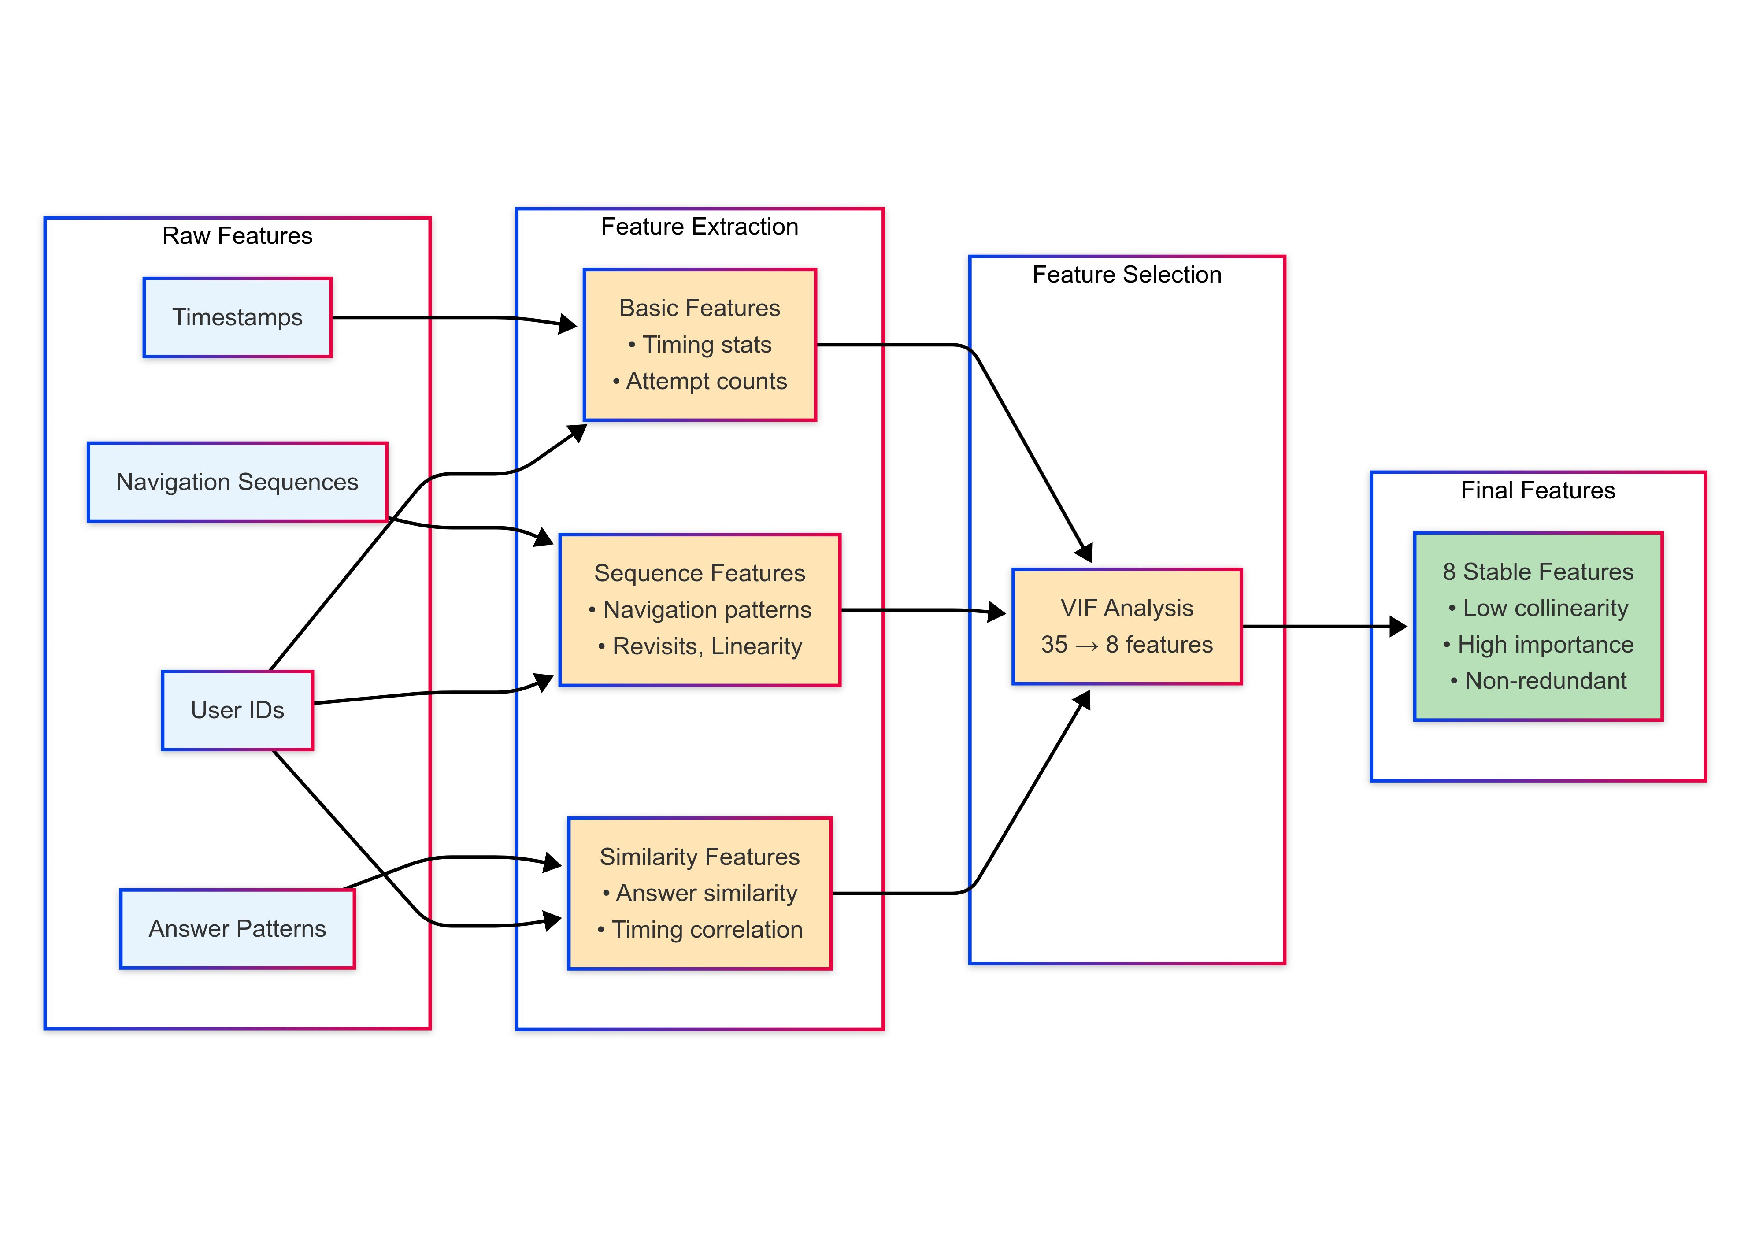
\includegraphics[width=0.9\textwidth]{figures/feature_engineering_process.pdf}
    \caption{Proses Reduksi Fitur: Dari 35 Fitur Awal menjadi 8 Fitur Stabil melalui Analisis VIF}
    \label{fig:feature_reduction_process}
\end{figure}

\subsubsection{Analisis Multikolinearitas dengan VIF}
\label{sec:analisisVIF}

Variance Inflation Factor (VIF) digunakan untuk mengidentifikasi redundansi antar fitur:

\begin{equation}
VIF_i = \frac{1}{1-R_i^2}
\end{equation}

dimana $R_i^2$ adalah coefficient of determination dari regresi fitur $i$ terhadap semua fitur lainnya.

Proses eliminasi iteratif:
\begin{enumerate}
    \item Hitung VIF untuk semua fitur
    \item Identifikasi fitur dengan VIF tertinggi
    \item Jika VIF $> 10$, eliminasi fitur tersebut
    \item Ulangi hingga semua VIF $< 10$
\end{enumerate}

Hasil analisis mengeliminasi 27 fitur redundan, menyisakan 8 fitur dengan VIF $<10$ yang memberikan informasi unik.

\subsubsection{Delapan Fitur Final untuk Model}
\label{sec:fiturFinal}

Setelah proses seleksi, 8 fitur stabil dengan kontribusi informasi maksimal:

\begin{table}[htbp]
\centering
\caption{Karakteristik 8 Fitur Final Hasil Seleksi VIF}
\label{tabel:fiturFinalKarakteristik}
\begin{tabular}{|p{5cm}|c|c|p{5cm}|}
\hline
\textbf{Nama Fitur} & \textbf{VIF} & \textbf{Importance} & \textbf{Interpretasi} \\
\hline
\texttt{max\_nav\_similarity\_zscore} & 4.87 & 0.245 & Z-score kemiripan navigasi maksimum, indikator utama koordinasi \\
\hline
\texttt{mean\_nav\_similarity\_zscore} & 3.98 & 0.218 & Rata-rata z-score kemiripan, mengukur konsistensi pola \\
\hline
\texttt{median\_step\_duration} & 3.24 & 0.156 & Median durasi langkah, \textit{robust indicator} kecepatan \\
\hline
\texttt{std\_nav\_similarity\_zscore} & 7.89 & 0.142 & Variabilitas kemiripan, mendeteksi selective cheating \\
\hline
\texttt{std\_step\_duration} & 3.41 & 0.098 & Konsistensi kecepatan pengerjaan \\
\hline
\texttt{nav\_revisits\_count} & 2.56 & 0.076 & Pola kunjungan ulang, indikator uncertainty \\
\hline
\texttt{quick\_actions\_count} & 5.12 & 0.045 & Aksi sangat cepat, possible copy-paste indicator \\
\hline
\texttt{sumgrades} & 6.23 & 0.020 & Nilai total, context untuk interpretasi \\
\hline
\end{tabular}
\end{table}

Kedelapan fitur ini mencakup semua aspek penting deteksi kecurangan: similarity (4 fitur), temporal patterns (2 fitur), navigation behavior (1 fitur), dan performance context (1 fitur). Kombinasi ini terbukti optimal dalam eksperimen dengan akurasi deteksi 98.33\%.
